\documentclass[a4paper, onecolumn, 12pt]{IEEEtran}
%\documentclass[draftcls, onecolumn, a4paper, twoside]{IEEEtran}


% These values get used many times, so it is easier to define then once here.
% Module code
\def\modulecode{ELI 220}
% Module name
\def\modulename{Linear Systems and Signals}
% Assessment title
\def\assessment{Practical 2}
\def\assessmenttitle{Passive RC, RL and RLC filter circuit
analysis}
% Group number
\def\groupnumber{43}

% Student details: (Leave blank the last student(s) if your group has fewer people. The contributions MUST add up to 100%. Additional rows in the table on the title page can be commented out in titlepage.tex.)
% Details of the first student
\def\firststudentname{Emma Muller}
\def\firststudentnumber{24875882}
\def\firststudentcontribution{33.3}
% Details of the second student
\def\secondstudentname{Jan-Hendrik Brink}
\def\secondstudentnumber{23694956}
\def\secondstudentcontribution{33.3}
% Details of the third student
\def\thirdstudentname{Sean van Wyk}
\def\thirdstudentnumber{24606872}
\def\thirdstudentcontribution{33.3}



% Allows multi-line equations to be split over a number of pages.
\interdisplaylinepenalty=2500 


\usepackage{amsmath}
\usepackage{amssymb}
\usepackage{cite}
\usepackage{graphicx}
\usepackage{lastpage}
\usepackage{listings}
\usepackage{minted}
\usepackage{multirow}
\usepackage{paralist}
\usepackage{placeins}  % For \FloatBarrier
%\usepackage{rotfloat}
\usepackage{rotating}
\usepackage[tight,small]{subfigure}  % normalsize small footnotesize
\usepackage{tabularx}
\usepackage{tabulary}
\usepackage{mdframed}
% I prefer this to the default font.
\usepackage{newtxmath}
% \usepackage{newtxtext}
\renewcommand{\rmdefault}{ntxtlf} 
%https://tex.stackexchange.com/questions/347566/math-digits-are-rendered-in-cm-when-using-libertine-and-newtxmath-with-xelatex-i


% Set the page format up.
\usepackage{geometry}
\geometry{includefoot}
\geometry{paper=a4paper}
\geometry{left=25mm}
\geometry{right=25mm}
\geometry{top=25mm}
\geometry{bottom=20mm}
\geometry{headsep=10mm}
\geometry{footskip=10mm}
%\geometry{columnsep=4mm}


\usepackage[pdftex]{hyperref}
%\hypersetup{pdfborder={0 0 0.2}}
\usepackage{xcolor}
\definecolor{darkred}{rgb}{0.8,0,0}
\definecolor{darkgreen}{rgb}{0,0.45,0}
\definecolor{darkblue}{rgb}{0,0,0.3}
\hypersetup{colorlinks=True, citecolor=black, filecolor=black, linkcolor=black, urlcolor=black}

% Set the PDF properties of the document.
\hypersetup{%
  pdftitle={\modulecode-- \assessment: \assessmenttitle},
  pdfauthor={Group \groupnumber}}


\usepackage[acronym,nonumberlist,nopostdot,style=super]{glossaries}  % This must be after hyperref.

% Load the abbreviations.
% \loadglsentries{abbreviations}
% \makeglossaries

% % Format the abbreviations list.
% \renewenvironment{theglossary}%
% {%\vspace{-1em}%
% \begin{supertabular}{ @{} l p{\textwidth} }}% Added @{} here to get left justification.
% {\end{supertabular}}
% \renewcommand{\acronymname}{\vspace{-1.2em}}%Abbreviations}
% %\renewcommand{\glspostdescription}{}
% \renewcommand{\glsgroupskip}{}


\usepackage{fancyhdr}
% Set the page format up.
\def\pagenumberfooter{\thepage}
\fancypagestyle{plain}{%
  \fancyhf{}
  \lhead{}
  \rhead{}
  \lfoot{}
%  \cfoot{Confidential}
  \rfoot{\thepage}
  \renewcommand{\headrulewidth}{0pt}
  \renewcommand{\footrulewidth}{0pt}
}
\def\pagenumberfooter{\thepage}
\fancypagestyle{fancy}{%
  \fancyhf{}
  \lhead{}
  \rhead{}
  \lfoot{\modulecode~-- \assessment~-- Group \groupnumber}
%  \cfoot{Confidential}
  \rfoot{Page~\thepage~of~\pageref{LastPage}}
  \renewcommand{\headrulewidth}{0pt}
  \renewcommand{\footrulewidth}{0.5pt}
}


\hyphenation{mono-pulse}
\hyphenation{retro-directive}



% \renewcommand{\Re}{\mathrm{R\hspace{-0.09em}e\hspace{-0.08em}}}
% \renewcommand{\Im}{\mathrm{I\hspace{-0.07em}m\hspace{-0.08em}}}
% I prefer this to the default versions - feel free to disagree.
\usepackage[cal=boondoxo]{mathalfa}
\renewcommand{\Re}{\mathcal{R\hspace{-0.2em}e\hspace{-0.1em}}}
\renewcommand{\Im}{\mathcal{I\hspace{-0.25em}m\hspace{-0.15em}}}

\newlength{\equalswidth}
\settowidth{\equalswidth}{$ =~ $}
\newcommand{\eqsplitline}{\nonumber \\ & \hspace{\equalswidth}}
\newcommand{\eqsplitaligned}{\\ & \hspace{\equalswidth}}


%\setlength{\parindent}{0cm}
\setlength{\parskip}{0.3em plus 0.3em minus 0.3em}


%\def\today{27 March 2018}
% Get the Day Month Year format.
\def\today{%
  \number\day
  \space
  \ifcase\month\or January\or February\or March\or April\or May\or
  June\or July\or August\or September\or October\or November\or
  December\fi
  \space
  \number\year
}


% Allow large floats.
\renewcommand\topfraction{1}
\renewcommand\bottomfraction{0}
\renewcommand\textfraction{0}
\renewcommand\floatpagefraction{1}
\setcounter{topnumber}{10}
\setcounter{totalnumber}{10}


% Increase the figure caption font size.
\usepackage[font=normalsize]{caption}

% Deal with missing images which are not directly included in the repository
\newcommand{\noimage}{%
  \fbox{\parbox[t][0.3\textwidth][c]{0.48\textwidth}{\centering Image file is missing.}}
%  \setlength{\fboxsep}{-\fboxrule}%
%  \fbox{\phantom{\rule{10pt}{10pt}}File missing\phantom{\rule{10pt}{10pt}}}% Framed box
}
\let\includegraphicsoriginal\includegraphics
\renewcommand{\includegraphics}[2][width=\textwidth]
{%
  \IfFileExists{#2}
  {\includegraphicsoriginal[#1]{#2}}%
  {\noimage}%
%  {\fbox{\includegraphicsoriginal[#1]{drawings/gripen}\makebox[0pt]{File #2 is missing.}}}%
}

% Centred column in tabularx.
\newcolumntype{Y}{>{\centering\arraybackslash}X}


\begin{document}


% Try to keep text inside the right margin.
\sloppy


% The language used in the source-code listings.
\lstset{language=Python}
\lstset{numbers=left}
\lstset{basicstyle=\small}
\lstset{breaklines=true, breakatwhitespace=false}
\lstset{xleftmargin=7mm,linewidth=\textwidth,xrightmargin=7mm}

% Colours for code listings.
\definecolor{codegreen}{RGB}{0,200,0}
\definecolor{codepurple}{RGB}{220,0,220}
\definecolor{codecyan}{RGB}{0,200,200}

\lstset{keywordstyle=\color{blue}}%\bfseries}
\lstset{commentstyle=\color{codegreen}}%\itshape}
\lstset{stringstyle=\color{red}}

% Variables.
\lstset{classoffset=2,morekeywords={input, output, beat}, keywordstyle=\color{orange}, classoffset=0}
% Function names.
\lstset{classoffset=3,morekeywords={choice},keywordstyle=\color{codepurple},classoffset=0}
% Classes.
\lstset{classoffset=4,morekeywords={random},keywordstyle=\color{codecyan},classoffset=0}

\setminted{fontsize=\small,xleftmargin=7mm,xrightmargin=7mm, breaklines, breakanywhere, linenos}
\renewcommand\theFancyVerbLine{\small\arabic{FancyVerbLine}}

% Customise the reference format.
\bstctlcite{IEEEexample:BSTcontrol}


% Title page
% Title page

\newcolumntype{A}{>{\centering\arraybackslash}m{4cm}}
\newcolumntype{B}{>{\centering\arraybackslash}m{3.75cm}}
\newcolumntype{C}{>{\centering\arraybackslash}m{3.25cm}}

\begin{titlepage}
    \begin{center}

        \vspace*{2cm}
    
        % University Logo
        
\includegraphics[width=0.6\textwidth]{drawings/up_logo_ebit.pdf}\\[2.0cm]    
    	
        % Department Title
        \textsc{\LARGE\bfseries \modulecode}\\[1.0cm]
    	
        % Module Tile
        \textsc{\Large\bfseries \modulename}\\[0.75cm]
    
        % Assignment Title
        \textsc{\large\assessment:~\assessmenttitle}\\[0.5cm]
        
        %Group Number
        \textsc{\large Group \groupnumber}\\[1.0cm]
        
    
        % Students/Contributors Table
        \begin{table}[h]
            \centering
            \normalsize
            \begin{tabularx}{\textwidth}{|A|C|B|C|}
                \hline
                \textbf{Name and Surname} & \textbf{Student Number} & \textbf{Signature} & \textbf{\% contribution} \\
                \hline
                \firststudentname   & \firststudentnumber   & & \firststudentcontribution \\ 
                & & &   \\ \hline 
                \secondstudentname  & \secondstudentnumber  & & \secondstudentcontribution \\ 
                & & &   \\ \hline 
                \thirdstudentname   & \thirdstudentnumber   & & \thirdstudentcontribution \\ 
                & & &   \\ \hline 
                % \fourthstudentname  & \fourthstudentnumber  & & \fourthstudentcontribution \\ 
                % & & &   \\ \hline 
            \end{tabularx}
        \end{table}
		
    \end{center}

  % Report Declaration
%   Comment this line out and uncomment the line below it in the \verb|report.tex| file to include the required declaration.
    \noindent By submitting this assignment we confirm that we have read and are aware of the University of Pretoria's policy on academic dishonesty and plagiarism and we declare that the work submitted in this assignment is our own as delimited by the mentioned policies. We explicitly declare that no parts of this assignment have been copied from current or previous students' work or any other sources (including the internet), whether copyrighted or not. We understand that we will be subjected to disciplinary actions should it be found that the work we submit here does not comply with the said policies.
	
	\vfill
    \begin{center}
		\large\today
    \end{center}

\end{titlepage}


%% Avoid expanding abbreviations.
%\glsunsetall
% Ensure that the abbreviations are expanded in the text.
% \glsresetall

% Table of Contents
\pagenumbering{roman}
\pagestyle{plain}
\setcounter{tocdepth}{2}
\addtocontents{toc}{\protect\thispagestyle{plain}}
\tableofcontents
\clearpage
\pagenumbering{arabic}
\setcounter{page}{1}
\pagestyle{fancy}


\section{Introduction}
\label{sec:introduction}
The analysis of linear time-invariant (LTI) circuits in both the time and frequency domains is a fundamental aspect of signal processing and communications engineering. Filters such as RC, RL and RLC circuits are widely used to shape signals, suppress unwanted frequency components, and control transient responses. Understanding their behavior provides the foundation for designing practical systems ranging from audio electronics to communication networks.

In this practical, the Fourier transform and impulse response analysis are applied to study how basic filter circuits respond to different input signals. The preparatory work focuses on deriving analytical expressions for transfer functions and impulse responses, and on examining the frequency-domain characteristics of periodic and pulse signals. The experimental work involves constructing circuits, measuring their outputs in the time and frequency domains using an oscilloscope, and comparing these results with theoretical predictions.

The objective of the report is to demonstrate the relationship between theory, simulation, and experiment, and to highlight how factors such as component values and damping influence the frequency and time responses of passive RC, RL, and RLC filters.


\newpage
\section{Preparatory Work}
\label{sec:prep_work}

\subsection{Deriving the Fourier Transform of a pulse train}
\label{subsec:cf}

A pulse train, $c(t)$, can be described as a single rectangular pulse convolved with a series of impulses given by \cite{lathi}
\begin{equation} \label{c(t)}
  c(t) = A\operatorname{rect}(\frac{t}{\tau}) \,\ast\, \sum_{n=-\infty}^{\infty} \delta(t-nT).
\end{equation}

The $rect$ function is a single rectangular pulse centred at $t=0\,$s, where $\tau$ is the width or duration of the pulse. In other words, the function is equal to $A$ (a real-valued number, the amplitude) in the interval $[\frac{-\tau}{2}, \frac{\tau}{2}]$, and 0 elsewhere. $\sum_{n=-\infty}^{\infty} \delta(t-nT)$ is known as an impulse train or Dirac Comb, made up of delta functions ($\delta(t)$) spaced at intervals of $T$. Each $\delta(t-nT)$ is an impulse at time $t=nT$ where $n$ is any integer (positive, negative or zero) and $T$ is the period between each impulse (or the space between pulses). \cite{lathi}

By convolving these two functions, a rectangular pulse is "placed" at each impulse location, as shown in Figure \ref{fig:pulsetrain}. Essentially, the impulse train acts like a sampler that repeats the rectangular pulse every $T$ units of time. The resulting pulse train is used as the input to each filter, therefore the frequency spectrum thereof should be known in order to determine its effect. The frequency spectrum can be obtained by using the Fourier Transform \cite{lathi},
\begin{equation}\label{fouriertransform}
  C(f) = \mathscr{F}(c(t)).
\end{equation}

\begin{figure}[h]
  \centering
  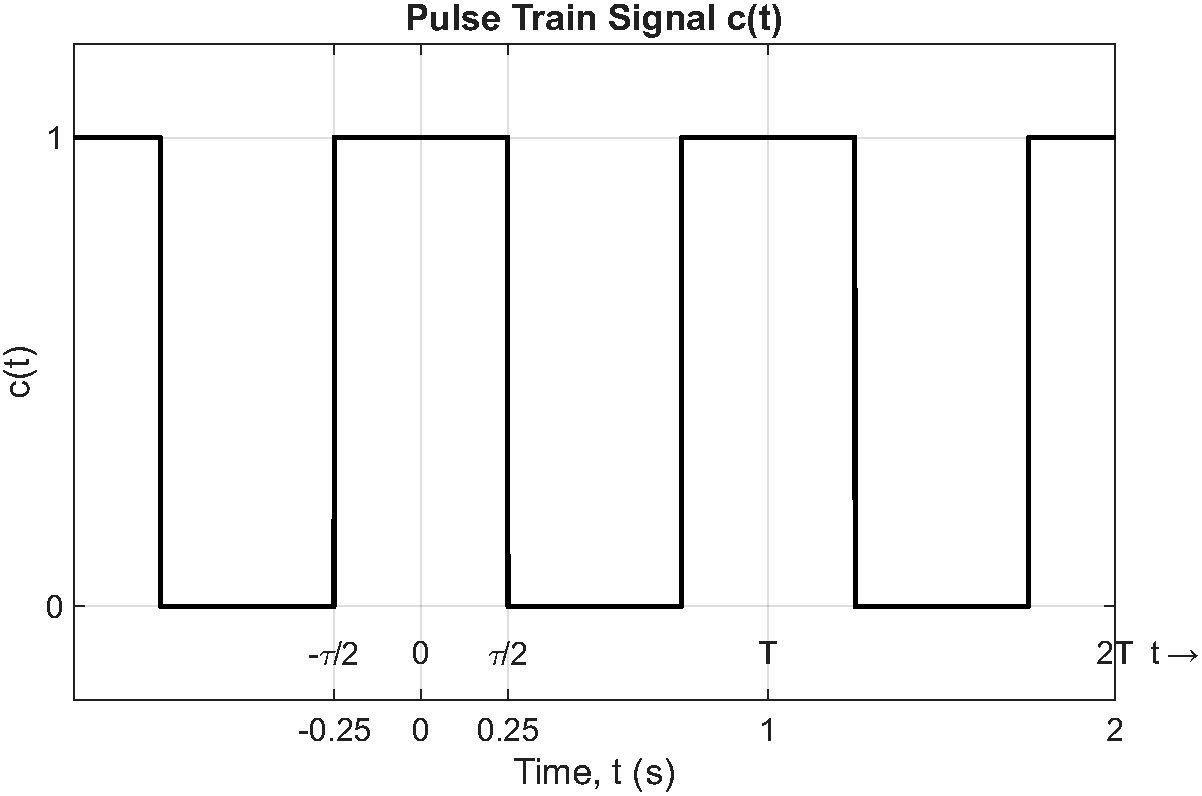
\includegraphics[width=0.8\textwidth]{plots/ct_plot.pdf}
  \caption{Pulse train $c(t)$}
  \label{fig:pulsetrain}
\end{figure}

For simplification purposes $C(\omega)$ will be used, where $\omega = 2\pi f$, with $f$ in Hz. The Fourier Transform itself also simplifies calculations, since convolution in the time domain is multiplication in the frequency domain (the convolution property) \cite{lathi}:
\begin{equation}\label{c_omega_base}
  C(\omega) = \operatorname{Rect}(\omega) \cdot \operatorname{Comb}(\omega),
\end{equation}
where $\operatorname{Rect}(\omega)$ is the transform of the rectangular pulse, and $\operatorname{Comb}(\omega)$ the transform of the impulse train. Their respective Fourier Tranform pairs are \cite{lathi}
\begin{equation} \label{rect_transformpair}
  \operatorname{Rect}(\frac{t}{\tau}) \overset{\mathcal{F}}{\longleftrightarrow} \tau\operatorname{sinc} (\frac{\omega \tau}{2}),
\end{equation}
where $\operatorname{sinc}(x)=\frac{\operatorname{sin}(x)}{x}$, and
\begin{equation}\label{comb_transformpair}
  \sum_{n=-\infty}^{\infty} \delta(t - nT) \overset{\mathcal{F}}{\longleftrightarrow} \frac{2\pi}{T} \sum_{k=-\infty}^{\infty} \delta(\omega - k\omega_0),
\end{equation}
where $\omega_0$ is $\frac{2\pi}{T}$ and $k$ is any real value and corresponds to a frequency component. \\
\\Combining (\ref{c_omega_base}), (\ref{rect_transformpair}) and (\ref{comb_transformpair}) results in 
\begin{equation} \label{c_omega}
  C(\omega) = \tau \operatorname{sinc}(\frac{\omega\tau}{2}) \cdot \frac{2\pi}{T} \sum_{k=-\infty}^{\infty} \delta(\omega - k\omega_0).
\end{equation}
Finally converting to $f$ in Hz
\begin{equation}
  C(f) = \tau\operatorname{sinc}(\frac{2\pi f\tau}{2}) \cdot \frac{2\pi}{T} \sum_{k=-\infty}^{\infty} \delta(2\pi f - \frac{k2\pi}{T})
\end{equation}
and then simplifying 
\begin{align} \label{cf_general}
  C(f) &= \tau\operatorname{sinc}(\pi f\tau) \cdot \frac{2\pi}{T}\sum_{k=-\infty}^{\infty}\frac{1}{2\pi}(\delta(f-\frac{k}{T})) \nonumber\\ 
       &= \frac{\tau}{T}\operatorname{sinc}(\pi f\tau) \cdot \sum_{k=-\infty}^{\infty}\delta(f-\frac{k}{T}).
\end{align}

The final result, equation (\ref{cf_general}) is the general formula for $C(f)$, the frequency spectrum of $c(t)$. Subsequently, multiple different cases can be applied and plotted as follows to further explore the results of $C(f)$.

\newpage

\subsubsection{$C(f)$ for $\tau = \frac{T}{2}$ and $T = 1\,s$}
By substituting the given values into equation (\ref{cf_general}) the equation:
\begin{equation}
  C(f) = \frac{1}{2} \operatorname{sinc} (\frac{\pi}{2}f)\sum_{k=-\infty}^{\infty}\delta(f-k)
\end{equation}
The plot of $C(f)$:
\begin{figure}[H]
  \centering
  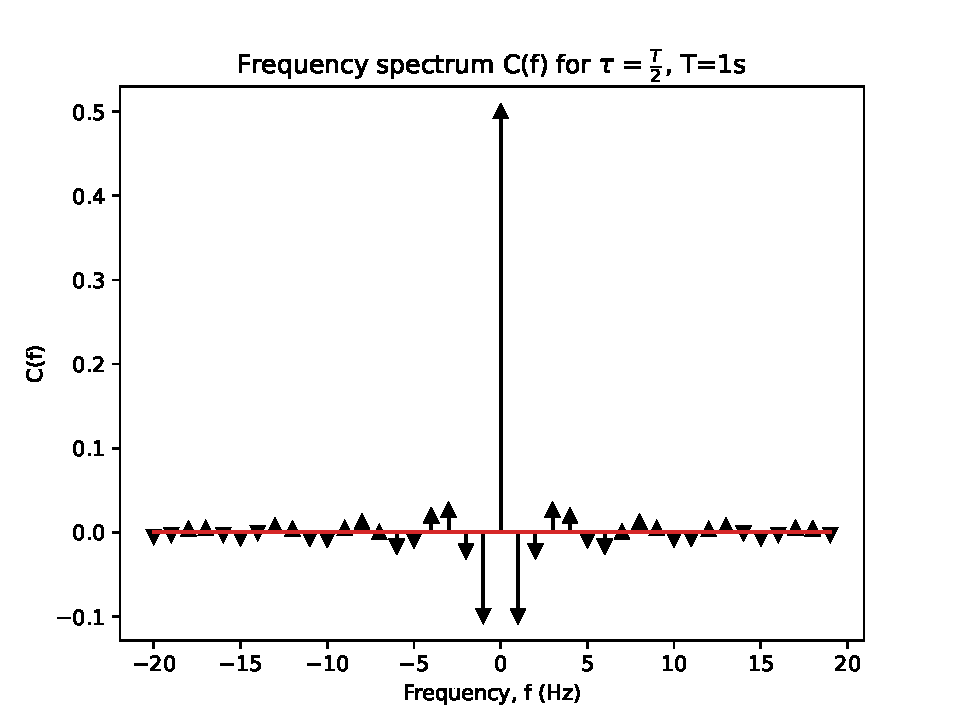
\includegraphics[width=0.8\textwidth]{plots/fig/Q1_a_C(f).pdf}
  \caption{Plot of $C(f)$ with $\tau=\frac{T}{2}$ and $T = 1s$, for $-20 < f < 20  \ Hz$ }
  \label{fig:Cf_1}
\end{figure}

\subsubsection{$C(f)$ for $\tau = \frac{T}{20}$ and $T = 1\,s$}
By substituting the given values into equation (\ref{cf_general}) the equation:
\begin{equation}
  C(f) = \frac{1}{20} \operatorname{sinc} (\frac{\pi}{20}f)\sum_{k=-\infty}^{\infty}\delta(f-k)
\end{equation}
The plot of $C(f)$:
\begin{figure}[H]
  \centering
  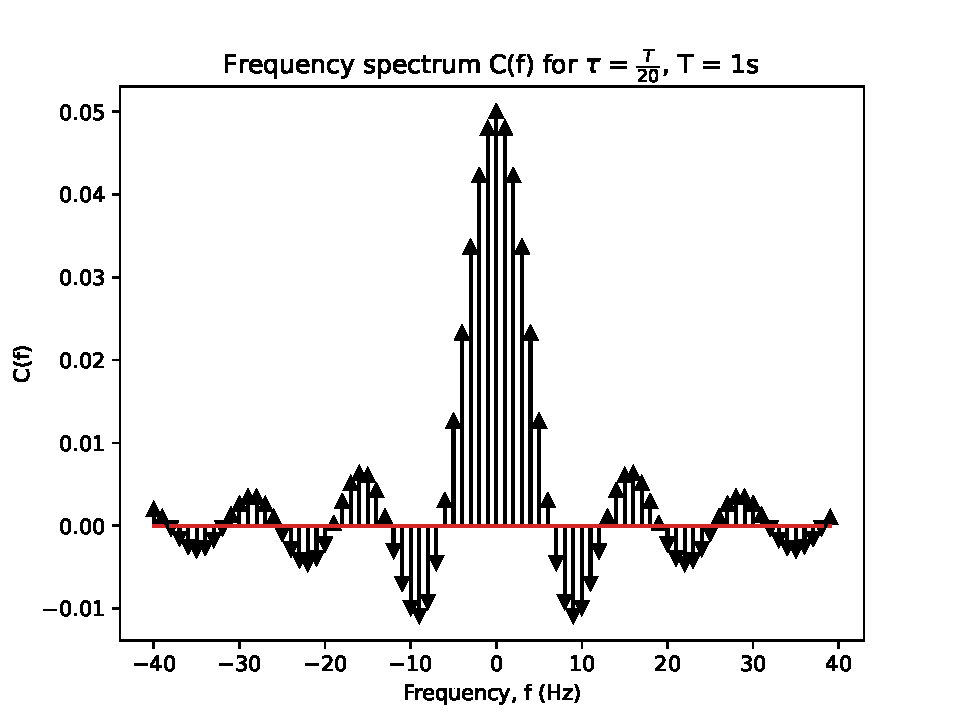
\includegraphics[width=0.8\textwidth]{plots/fig/Q1_b_C(f).pdf}
  \caption{Plot of $C(f)$ with $\tau=\frac{T}{2}$ and $T = 1s$, for $-40 < f < 40  \ Hz$ }
  \label{fig:Cf_2}
\end{figure}

\subsubsection{$C(f)$ for $\tau \to 0$ and $T = 1\,s$}

As the value of $\tau$ tends to 0, $\operatorname{rect}(\frac{t}{\tau})$ from the original equation for $c(t)$ (\ref{c(t)}), becomes narrower, eventually appearing as an impulse. Subsequently,
\begin{align}
  \operatorname{sinc}(\pi f\tau) &= \frac{\operatorname(\pi f\tau)}{\pi f \tau} \nonumber\\
                                 &\approx \frac{\pi f \tau}{\pi f \tau}\nonumber\\ 
                                 &= 1 \nonumber
\end{align}
due to $\operatorname{sin}(x)$ being approximately equal to $x$ at small angles. This results in (\ref{cf_general}) simplifying to 
\begin{equation}
  C(f) = \frac{\tau}{T} \cdot \sum_{k=-\infty}^{\infty} \delta(f - \frac{k}{T}),
\end{equation}
but since $\tau \to 0$, $\frac{\tau}{T}$ also tends to 0. This leads to issues, since anything multiplied by zero is zero. So, the limit is rather taken and L'Hospital's rule applied to the indeterminate form of the sinc function, eventually resulting in 
\begin{align} \label{cf_tau->0}
  C(f) &= \frac{1}{T} \cdot \sum_{k=-\infty}^{\infty} \delta(f - \frac{k}{T})\nonumber\\
       &= \sum_{k=-\infty}^{\infty} \delta(f - k),
\end{align}
since $T=1\,s$.

This result is an impulse train with an impulse of height 1 at each $f = k\,$Hz, shown in Figure \ref{fig:cf_tau->0}. Here $k=0$ is the "DC" value, $k=1$ is the fundamental frequency component, $k=2$ is the second harmonic, and so on.

\begin{figure}[h]
  \centering
  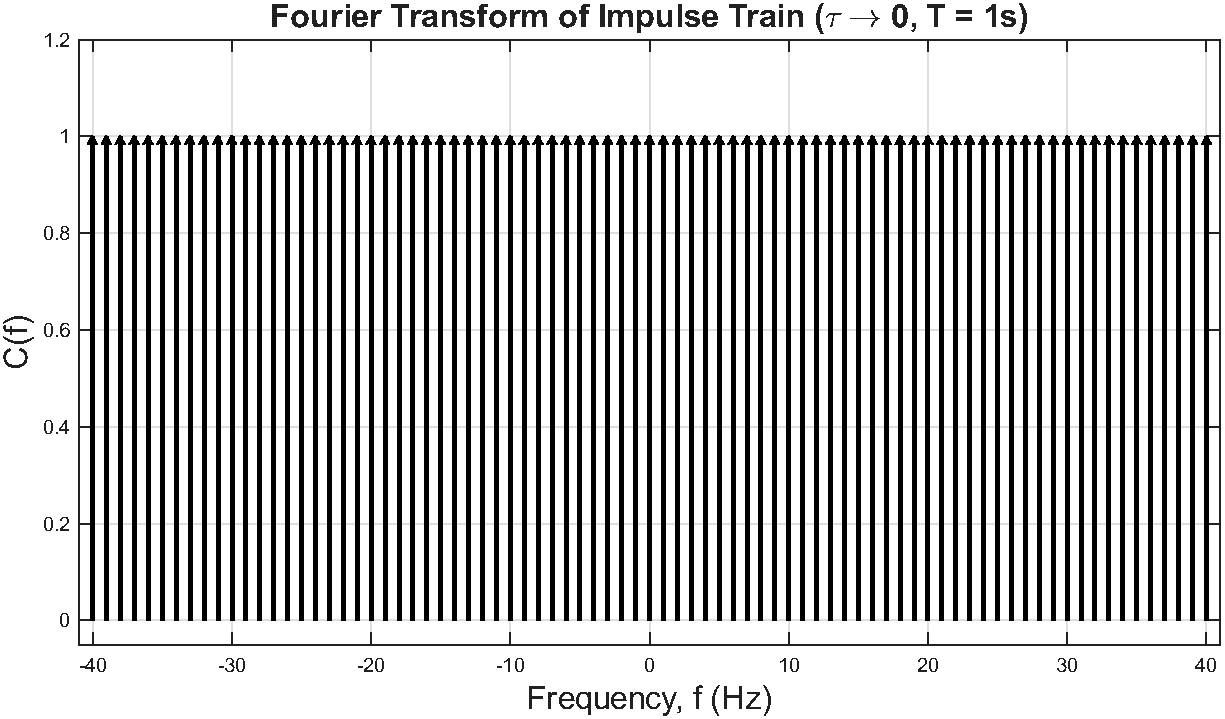
\includegraphics[width=0.8\textwidth]{plots/Q1c_plot.pdf}
  \caption{Plot of $C(f)$ with $\tau \to 0$ and $T = 1\,s$, for $-40 < f < 40\,$Hz}
  \label{fig:cf_tau->0}
\end{figure}

\subsubsection{$C(f)$ for $\tau = 75\,\mu s$ and $T = 3.7\,ms$}
By substituting the given values into equation (\ref{cf_general}) the equation:
\begin{equation}
  C(f) = \frac{75 \times 10^{-6}}{3.7 \times 10^{-3}} \operatorname{sinc} ( \pi f 75 \times 10^{-6}) \sum_{k=-\infty}^{\infty} \delta(f - \frac{k}{3.7 \times 10^{-3}})
\end{equation}
The plot of $C(f)$:
\begin{figure}[H]
  \centering
  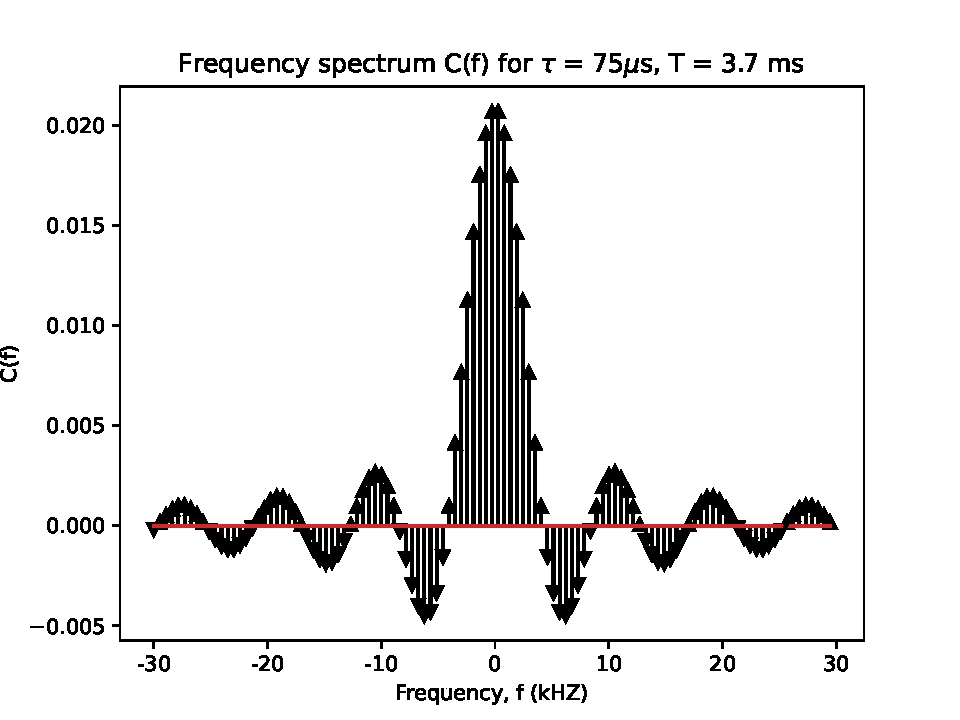
\includegraphics[width=0.8\textwidth]{plots/fig/Q1_d_C(f).pdf}
  \caption{Plot of $C(f)$ with $\tau=75 \mu s$ and $T = 3.7 ms$, for $-40 < f < 40  \ kHz$ }
  \label{fig:Cf_4}
\end{figure}

\subsection{Theoretical background on passive filters}
\label{subsec:theory_filter}
RC, RL, and RLC circuits function as passive filters, which means they can shape signals without requiring an external power source for amplification. Filters are electronic circuits designed to control the frequency content of a signal by allowing certain frequency ranges to pass while attenuating others. This selective behavior is achieved through the use of reactive components, such as capacitors and inductors, whose impedance varies with frequency. By exploiting this frequency-dependent impedance, these components enable the implementation of low-pass, high-pass, band-pass, or band-stop filters depending on the desired application. 

To construct a low-pass filter, a resistor is combined with a reactive component that presents high impedance at low frequencies, like a capacitor. In this practical, a $33\,nF$ capacitor is used. The capacitive reactance is defined as
\begin{equation} \label{X_c}
  X_c = \frac{1}{2 \pi f C}.
\end{equation}
From this expression, it is clear that the impedance of a capacitor decreases as the frequency increases. At low frequencies, the capacitor's impedance is high and it behaves like an open circuit, forcing most of the input signal to appear at the output. At high frequencies, the impedance becomes small, effectively shorting the signal to ground and preventing it from reaching the output. Thus, the RC circuit functions as a low-pass filter, passing frequencies below a certain threshold. The cutoff frequency is given by
\begin{equation}
\label{eqn:rc_cutoff}
f_L = \frac{1}{2\pi RC},
\end{equation}
at which the output signal power is reduced to half of its input value (the $-3\,$dB point).

A high-pass filter can be constructed by combining a resistor with a reactive component that exhibits low impedance at high frequencies. In this practical, a $10\,mH$ inductor is used. The inductive reactance is expressed as
\begin{equation}
\label{eqn:X_L}
X_L = 2 \pi f L.
\end{equation}
Since the impedance of the inductor increases with frequency, it blocks high-frequency signals while allowing low-frequency signals to pass through to ground. At low frequencies, the inductor behaves like a short circuit, diverting the signal away from the output. At high frequencies, its impedance is large, forcing the signal through the output node. The cutoff frequency for the RL high-pass filter is given by
\begin{equation} \label{rl_cutoff}
  f_H = \frac{R}{2 \pi L},
\end{equation}
where signals above $f_H$ are passed with their output power reduced to half at the cutoff.

A band-pass filter allows only a range of frequencies to pass while attenuating signals outside this range. It can be implemented by combining a low-pass and a high-pass filter. In this practical, an RLC circuit is used, consisting of a resistor, capacitor ($33\,nF$), and inductor ($10\,mH$). The resistor provides damping, which controls the sharpness of the resonance. \footnote{An additional measure often used is the quality factor $Q = \tfrac{1}{R}\sqrt{\tfrac{L}{C}}$, 
which describes the selectivity of the circuit around its resonant frequency. 
High $Q$ (small $R$) produces a sharp resonance cusp and narrow bandwidth, 
while low $Q$ (large $R$) flattens the response. \cite{lathi}} The lower and upper cutoff frequencies are determined by (\ref{eqn:rc_cutoff}) and (\ref{rl_cutoff}), while the bandwidth, defined as the range of frequencies passed by the filter, is
\begin{equation}
  \label{eqn:rlc_bw}
  BW = f_H - f_L.
\end{equation}
The center frequency, which lies at the midpoint of the passband is given by
\begin{equation}
  \label{eqn:rlc_center}
  f_C = \frac{1}{2 \pi \sqrt{LC}}.
\end{equation}

\subsection{Determining the time domain response of RC, RL and RLC circuits}
\label{subsec:ht_hf}

RC, RL, and RLC circuits are examples of linear, time-invariant systems \cite{lathi}. For such systems, the output is the convolution of the input signal, $x(t)$, with the impulse response, $h(t)$:
\begin{align}
  y(t) &= x(t) \ast h(t)\nonumber\\ 
       &= \int_{-\infty}^{\infty}x(\tau)h(t-\tau)d\tau,
\end{align}
where $x(t)$ is the output of the signal generator circuit used in Section \ref{sec:prac_results}. 

To better understand how filters affect signals, it is often convenient to work in the frequency domain. The frequency-domain represesntation is given by
\begin{equation}
  Y(f) = X(f) \cdot H(f),
\end{equation}
where
\begin{equation}
  \label{eqn:Hf}
  H(f) = \frac{Y(f)}{X(f)},
\end{equation}
and $|H(f)|$ represents the magnitude response of the filter.

In the frequency domain, circuit elements are expressed by their impedances \cite{ebn}:
\begin{align}
  Z_R &= R, \nonumber\\
  Z_L &= j\omega L = j2\pi fL, \nonumber\\ 
  Z_C &= \frac{1}{j\omega C} = \frac{1}{j2\pi fC}.
\end{align}

Using these expressions, transfer functions are conveniently derived in the Laplace domain with $s = j\omega$ or $j2\pi f$:
\begin{align}\label{laplace}
  H(s) &= \frac{V_{out}(s)}{V_{in}(s)} \nonumber\\ 
       &= \frac{Z_{out}}{Z_{total}}.
\end{align}
Here, $Z_{out}$ is the impedance across which the output is measured, and $Z_{total}$ is the total circuit impedance.

The circuits in Figures \ref{fig:RC_circuit} and \ref{fig:RL_circuit} are first-order circuits since the highest derivative in their governing equations is of order one. In other words, the voltage-current relationship can be described by a first-order differential equation. This property arises from the presence of a single energy storage element - either a capacitor in the RC circuit or an inductor in the RL circuit \cite{ebn}. In these systems $x(t)$ respresents the input voltage as a function of time, while $y(t)$ denotes the ouput voltage across the reactive component as a function of time.

\begin{figure}[h]
    \centering
    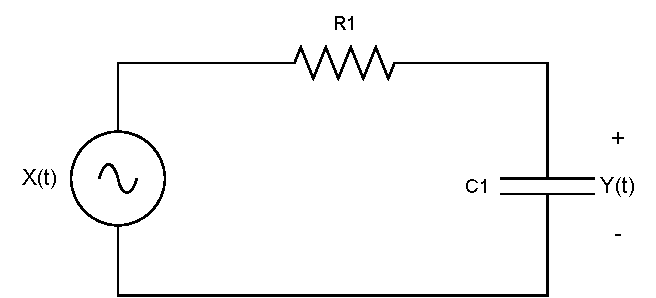
\includegraphics[width=0.8\textwidth]{Figures/RC.pdf}
    \caption{A series RC circuit}
    \label{fig:RC_circuit}
\end{figure}

\begin{figure}[h]
    \centering
    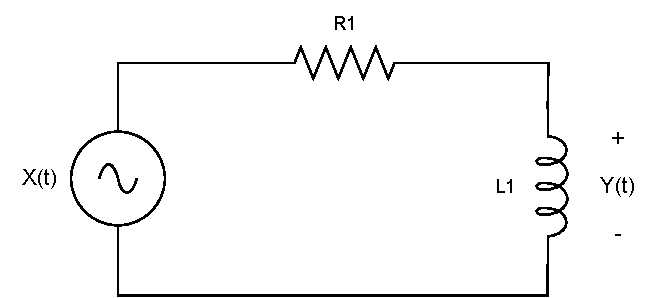
\includegraphics[width=0.8\textwidth]{Figures/RL.pdf}
    \caption{A series RL circuit}
    \label{fig:RL_circuit}
\end{figure}

Applying Kirchhoff's Voltage Law (KVL) \cite{ebn} to Figure \ref{fig:RC_circuit} yields
\begin{equation}
  x(t) = RC \cdot \frac{dy(t)}{dt} + y(t).
\end{equation}
Taking the Laplace transform and rearranging:
\begin{equation}
  \label{eqn:rc_Hs}
  H(s) = \frac{Y(s)}{X(s)} = \frac{1}{RCs+ 1}.
\end{equation}
The corresponding impulse is
\begin{equation} \label{eqn:rc_ht_general}
  h(t) = \frac{1}{RC} \cdot \mathrm{e}^{-\frac{t}{RC}}u(t),
\end{equation}
and the magnitude frequency response is 
\begin{equation}
  \label{eqn:rc_Hf_general}
  |H(f)| = \sqrt{\frac{1}{(2\pi RCf + 1)^2}}.
\end{equation}
From KVL, the governing equations of the RL circuit (Figure \ref{fig:RL_circuit}), are
\begin{align}
  x(t) &= Ri(t) + y(t), \label{eqn:rl_xt} \\ 
  y(t) &= L\frac{di(t)}{dt}. \label{eqn:rl_yt}
\end{align}
Taking the Laplace transform and eliminating $i(t)$:
\begin{equation}
  \label{eqn:rl_Hs}
  H(s) = \frac{Y(s)}{X(s)} = \frac{Ls}{R+Ls},
\end{equation}
which simplifies to
\begin{equation}
  \label{eqn:rl_Hs_2}
  H(s) = \frac{s}{\tfrac{R}{L} + s}.
\end{equation}
The impulse response is then
\begin{equation}
  \label{eqn:rl_ht_general}
  h(t) = \delta(t)-\frac{R}{L} \cdot \mathrm{e}^{-\tfrac{R}{L}t}u(t),
\end{equation}
and the magnitude frequency response is
\begin{equation}
  \label{eqn:rl_Hf_general}
  |H(f)| = \sqrt{\frac{(2 \pi fL)^2}{(R+2\pi fL)^2}}
\end{equation}

\begin{figure}[h]
  \centering
  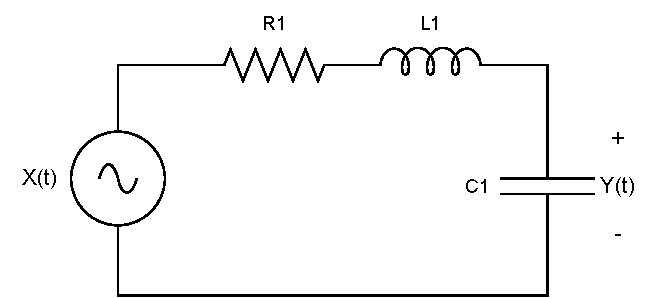
\includegraphics[width=0.8\textwidth]{Figures/RLC.pdf}
  \caption{Series RLC circuit}
  \label{fig:RLC_circuit}
\end{figure}

For the series RLC circuit in Figure \ref{fig:RLC_circuit}, KVL gives:
\begin{equation}
  \label{eqn:rlc_kvl_raw}
  x(t) = L\frac{di(t)}{dt} +  Ri(t) + \frac{1}{C}i(t)dt.
\end{equation}
Taking the Laplace Transform:
\begin{equation}
  H(s) = \frac{Y(s)}{X(s)} = \frac{1}{LCs^2 + RCs + 1}.
\end{equation}
The magnitude frequency response of the RLC circuit is then obtained by substituting $s = j 2 \pi f$:
\begin{equation}
  \label{eqn:rlc_Hf_general}
  |H(f)| = \frac{1}{\sqrt{ \left( 1 - (2 \pi f)^2 LC \right)^2 + j(2 \pi f RC)^2 }}.
\end{equation}

The general impulse response depends on the damping factor \cite{ebn}
\begin{equation}\label{alpha}
  \alpha = \frac{R}{2L}
\end{equation}
and the natural frequency 
\begin{equation} \label{omega_0}
\omega_0 = \frac{1}{\sqrt{LC}}.
\end{equation}
In the case of an underdamped RLC circuit($\alpha < \omega_0$)
\begin{equation} 
  \label{eqn:rlc_ht_general}
  h(t) = \frac{1}{\sqrt{\tfrac{1}{LC} - \left(\tfrac{R}{L}\right)^2}} \mathrm{e}^{-\tfrac{R}{L} t} \sin\!\Bigg(\sqrt{\tfrac{1}{LC} - \left(\tfrac{R}{L}\right)^2} \, t\Bigg) u(t).
\end{equation}
Furthermore, in the case of an overdamped circuit where $\alpha > \omega_0$:
\begin{equation}
  \label{eqn:rlc_ht_overdamped}
  h(t) = A e^{s_1 t} + B e^{s_2 t},
\end{equation}
with the characteristic roots of
\begin{equation}
  \label{char_roots}
  s_{1,2} = -\alpha \pm \sqrt{\alpha^2 - \omega_0^2}.
\end{equation}
In the critically damped case $\alpha = \omega_0$ and the two characteristic roots coincide:
\begin{equation}
  s_{1,2} = -\alpha = -\frac{R}{2L},
\end{equation}
and the impulse response for this case takes the form
\begin{equation} 
  \label{eqn:rlc_ht_critdamped}
  h(t) = (A + Bt) e^{-\alpha t} u(t).
\end{equation}
The constants $A$ and $B$ are determined via simultaneous equations from initial conditions of the system \cite{ebn}.

%========================================RC=Begin=======================================
\subsubsection{RC with $R_{RC} = 10\,k\Omega$ and $C = 33\,nF$} \strut \newline
Substituting the given values for $R$ and $C$ into equation (\ref{eqn:rc_ht_general}) yields:
\begin{equation}
  \label{eqn:rc_ht_sub}
  h(t) = \frac{1}{10000 \cdot 33 \times 10^{-9}} \cdot \mathrm{e}^{-\frac{t}{10000 \cdot 33 \times 10^{-9}}}u(t).
\end{equation}
Then plotting equation (\ref{eqn:rc_ht_sub}) for $ 0 \le t \le 1.5 \, ms$ yields Figure \ref{fig:RC_time}, an inverse exponential graph, which represents the time-domain response of the RC circuit. The voltage over the capacitor at time $ t= 0.0 \, ms$ is the maximum voltage, and as the capacitor discharges over time, the voltage difference over the capacior gets smaller, until at $t = 1.5 \, ms$ the voltage difference become negligibly small.
\begin{figure}[H]
  \centering
  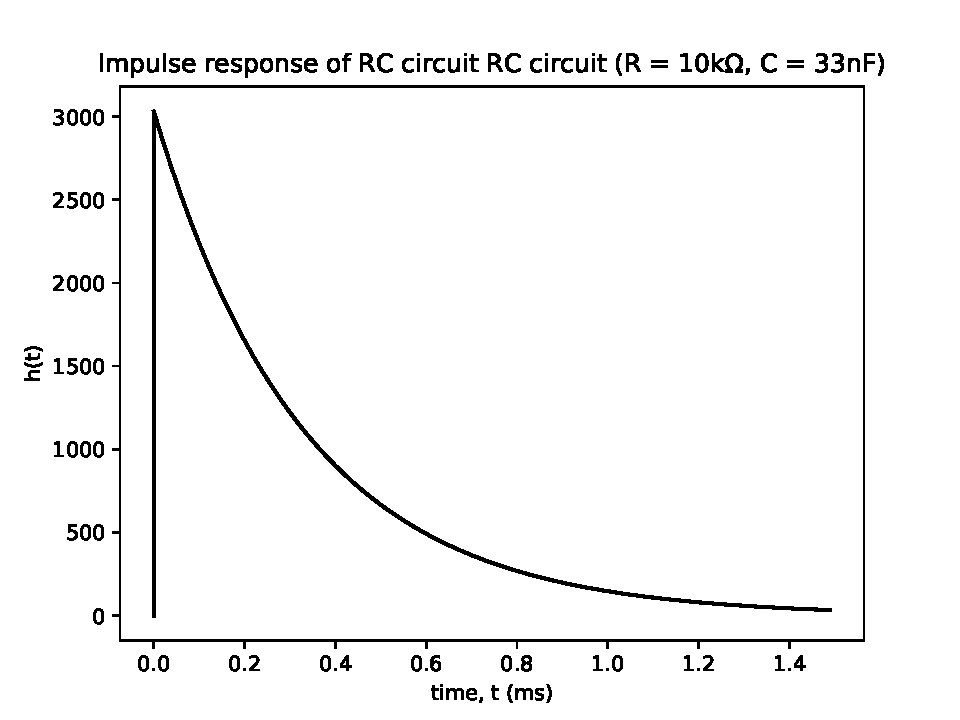
\includegraphics[width=0.78\textwidth]{plots/fig/Q2_a_RC_time.pdf}
  \caption{Plot of $h(t)$ with $R = 10\,k\Omega$ and $C=33\,nF$ for $ 0 \le t \le 1.5 \, ms$.}
  \label{fig:RC_time}
\end{figure}
Then substituting the given values for $R$ and $C$ into equation (\ref{eqn:rc_Hf_general}) yields:
\begin{equation}
  \label{eqn:rc_Hf_sub}
  |H(f)| = \sqrt{\frac{1}{(2\pi \cdot 10000 \cdot 33 \times 10^{-9} \cdot f + 1)^2}}.
\end{equation}
Plotting equation (\ref{eqn:rc_Hf_sub}) for $1\,Hz \le f \le 1\,MHz$, on a bode plot where the top graph is the magnitude spectrum in $dB$. This represents the magnitude of the frequency response of the RC circuit. The bottom graph is the phase spectrum in $Hz$ plotted on a logarithmic scale. This represents the phase change of the frequency response of the RC-circuit low pass filter.
The magnitude increases at higher frequencies, thus greatly decreasing the impedance and allowing the signal of a high frequency to short circuit through the capacitor. Thus only the low frequency signals are allowed through the output circuit.
\begin{figure}[H]
  \centering
  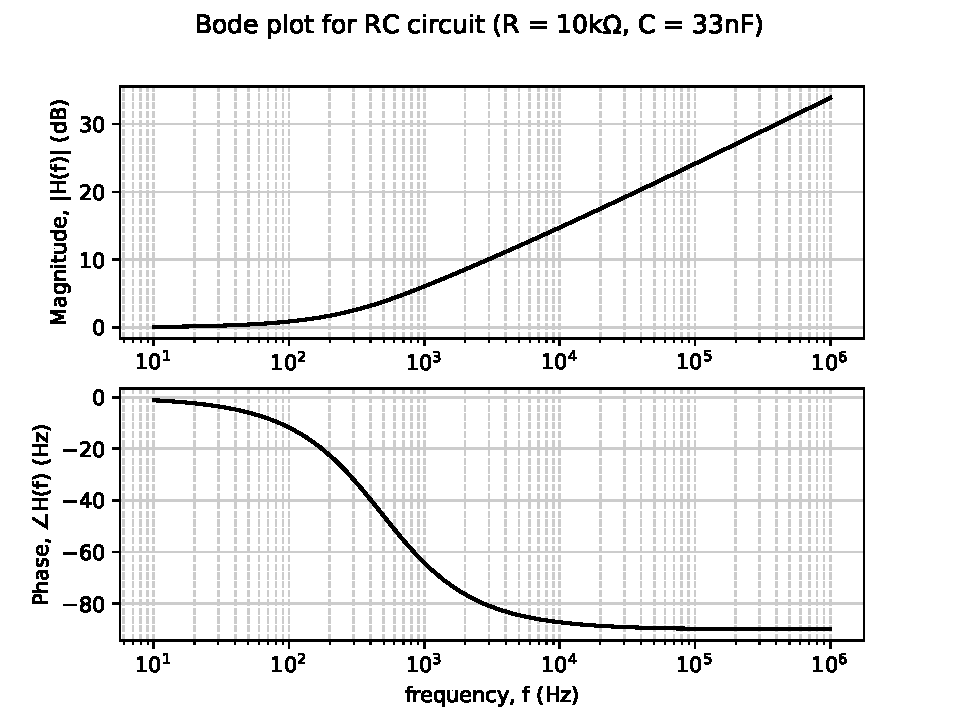
\includegraphics[width=0.78\textwidth]{plots/fig/Q2_a_RC_freq.pdf}
  \caption{Plot of $|H(f)|$ with $R = 10\,k\Omega$ and $C=33\,nF$ for $ 1\,Hz \le t \le 1\,MHz$.}
  \label{fig:RC_freq}
\end{figure}
%========================================RC=End=======================================

%========================================RL=Begin=======================================
\subsubsection{RL with $R_{RL} = 56\,\Omega$ and $L = 10\,mH$} \strut \newline
Similarly, substituting the given values for $R$ and $L$ into equation (\ref{eqn:rl_ht_general}) yields:
\begin{equation}
    \label{eqn:rl_ht_sub}
    h(t) = \delta(t)-\frac{56}{0.01} \cdot \mathrm{e}^{-\tfrac{56}{0.01}t}u(t),
\end{equation}
Furthermore, plotting equation (\ref{eqn:rl_ht_sub}) for $ 0 \le t \le 2 \, ms$ results in  the following inverse exponential graph, which represents the time-domain response of the RL-circuit, high-pass filter. The inductor voltage at $t = 0.0 \, ms$ is the maximum voltage. As the inductor charges over time, the voltage difference over the inductor decreases until it becomes negligibly small (like at $t = 2.0 \, ms$).
\begin{figure}[H]
  \centering
  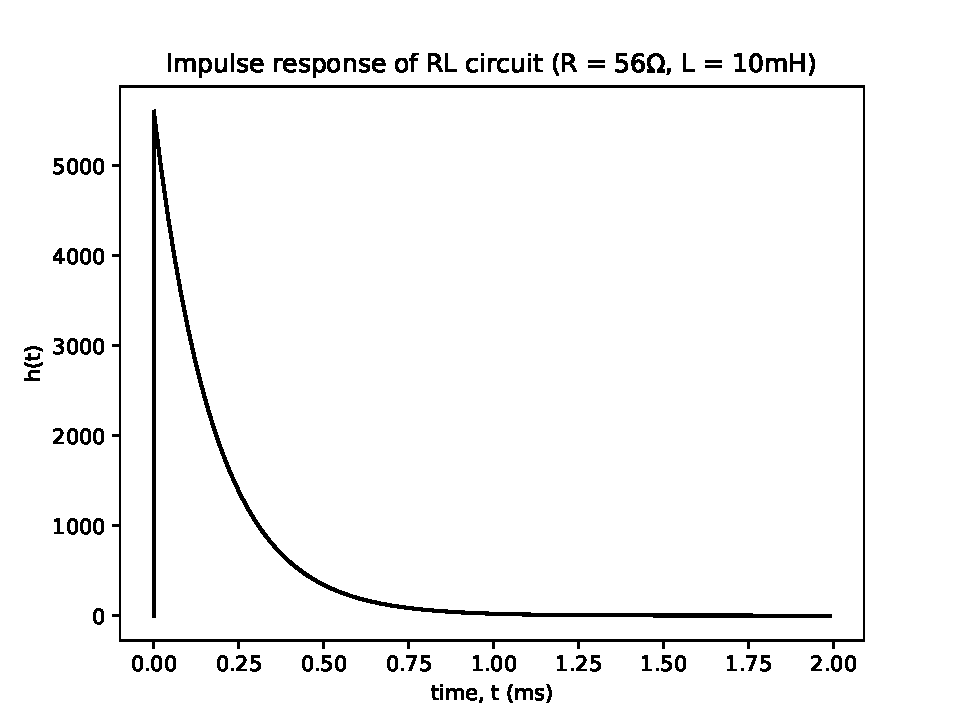
\includegraphics[width=0.78\textwidth]{plots/fig/Q2_b_RL_time.pdf}
  \caption{Plot of $h(t)$ with $R = 56\,\Omega$ and $L=10\,mH$ for $ 0 \le t \le 2 \, ms$.}
  \label{fig:RL_time}
\end{figure}
Then substituting the given values into equation (\ref{eqn:rl_Hf_general}) results in:
\begin{equation}
  \label{eqn:rl_Hf_sub}
  |H(f)| = \sqrt{\frac{(2 \pi f(0.01))^2}{(56+2\pi f(0.01))^2}}
\end{equation}
Plotting equation (\ref{eqn:rc_Hf_sub}) as a bode plot for $1\,Hz \le f \le 100\,MHz$, has Figure \ref{fig:RL_freq} as a result.

The magnitude decreases at higher frequencies, where the impedance increases and thereby forcing the signal through the output circuit. Only the high frequency components of the signal pass through the output circuit.
\begin{figure}[H]
  \centering
  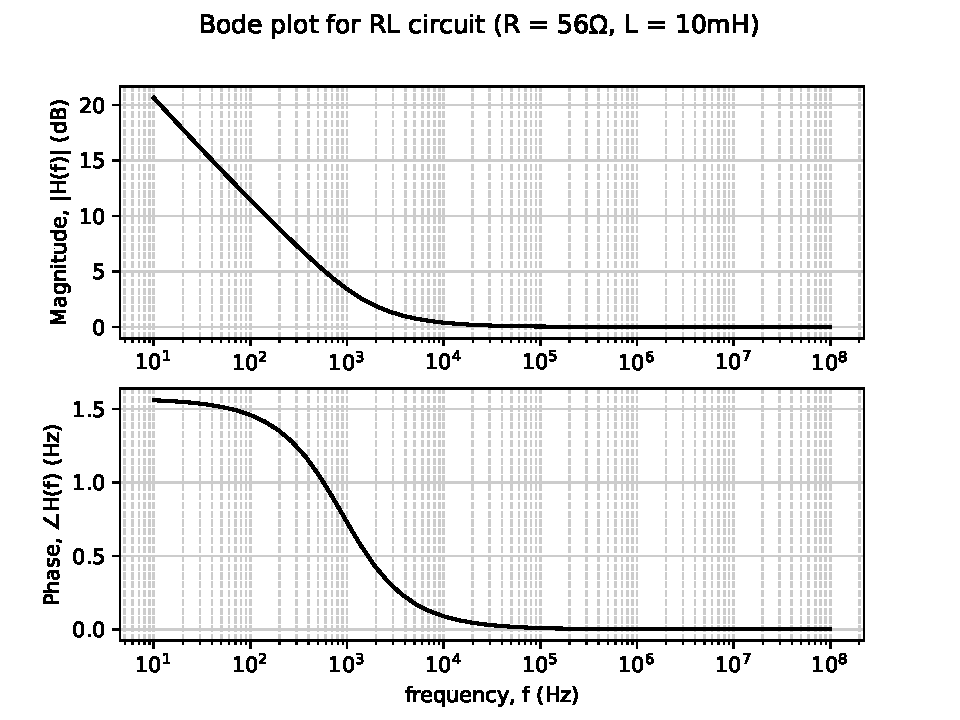
\includegraphics[width=0.78\textwidth]{plots/fig/Q2_b_RL_freq.pdf}
  \caption{Plot of $|H(f)|$ with $R = 56\,\Omega$ and $L=10\,mH$ for $ 1\,Hz \le t \le 100\,MHz$.} 
  \label{fig:RL_freq}
\end{figure}
%========================================RL=End=======================================

%========================================RLC_0=Begin=======================================
\subsubsection{RLC with $R_{RLC} = 0\,\Omega$, $C=33\,nF$ and $L=10\,mH$} 
In this case ($\alpha = 0$ and $\omega_0 =  55\,048.2$) It is evident that this is an underdamped response ($\alpha < \omega_0$). Substituting The given values into equation (\ref{eqn:rlc_ht_general}) results in
\begin{equation}
  \label{eqn:rlc_0_ht_sub_intermediate}
  h(t) = \frac{1}{\sqrt{\tfrac{1}{(0.01)(33 \times 10^{-9})} - \left(0\right)^2}} \mathrm{e}^{-(0) t} \sin\!\Bigg(\sqrt{\tfrac{1}{(0.01)(33 \times 10^{-9})} - \left(0\right)^2} \, t\Bigg) u(t),
\end{equation}
which simplifies to:
\begin{equation}
  \label{eqn:rlc_0_ht_sub}
  h(t) = 18.166 \times 10^{-6} \sin(55047.89 \, t).
\end{equation}
Plotting this result for $ 0 \le t \le 4 \, ms$ yields a sinusoidal graph in Figure \ref{fig:RLC_0_time}. This is an extremely underdamped response since the $0\,\Omega$ resistor does not dissipate any power. The signal oscilates indefinitely between the capacitor and inductor. In practice it cannot oscilate infinitely since some power is dissipated by the internal resistance of the wire.
\begin{figure}[H]
  \centering
  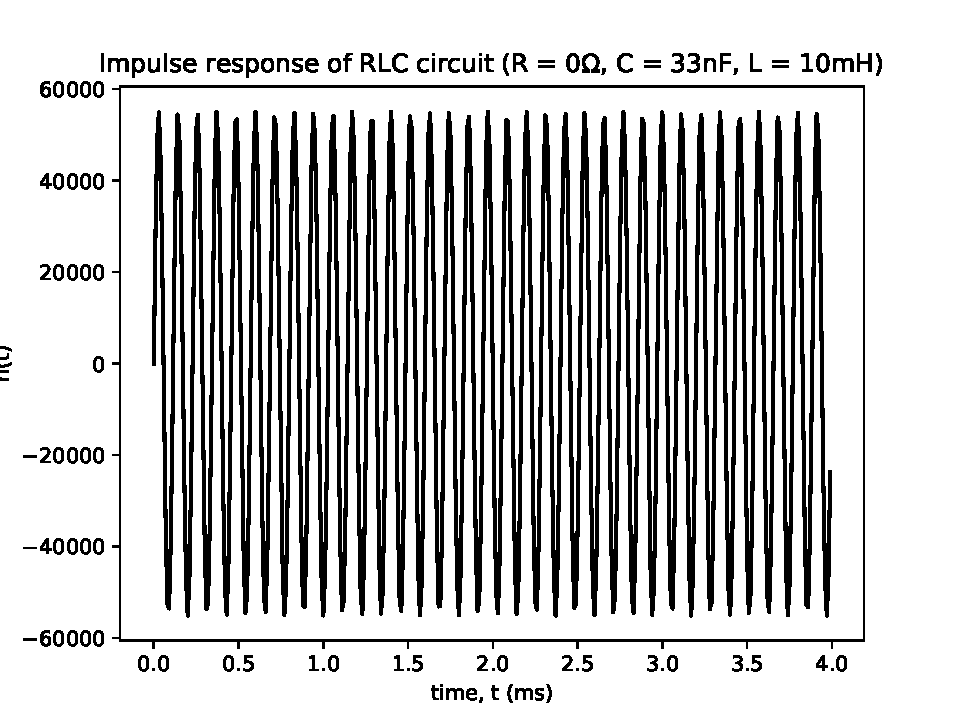
\includegraphics[width=0.76\textwidth]{plots/fig/Q2_c_RCL_0_time.pdf}
  \caption{Plot of $h(t)$ with $R = 0\,\Omega$, $L=10\,mH$ and $C=33\,nF$ for $ 0 \le t \le 4 \, ms$.}
  \label{fig:RLC_0_time}
\end{figure}
For the frequency response, the given values were substituted into (\ref{eqn:rlc_Hf_general}):
\begin{equation}
  \label{eqn:rlc_0_Hf_sub_intermediate}
    |H(f)| = \frac{1}{\sqrt{ \left( 1 - (2 \pi f)^2 (0.01)(33 \times 10^{-9}) \right)^2 + (2 \pi f (0)(33 \times 10^{-9}))^2 }}.
\end{equation}
Simplifying:
\begin{equation}
   \label{eqn:rlc_0_Hf_sub}
    |H(f)| = \frac{1}{\sqrt{ \left( 1 - (2 \pi f)^2 (0.01)(33 \times 10^{-9}) \right)^2}}. 
\end{equation}
Plotting for $1\,Hz \le f \le 1\,MHz$, on a bode plot results in Figure \ref{fig:RLC_0_freq}. It can be noted that the magnitude spectrum forms a cusp where the phase spectrum suddenly changes from $0$ to $-\pi$. The frequency at this point is the resonant frequency where the RLC circuit band-filter transitions from capacitive to inductive qualities.
\begin{figure}[H]
  \centering
  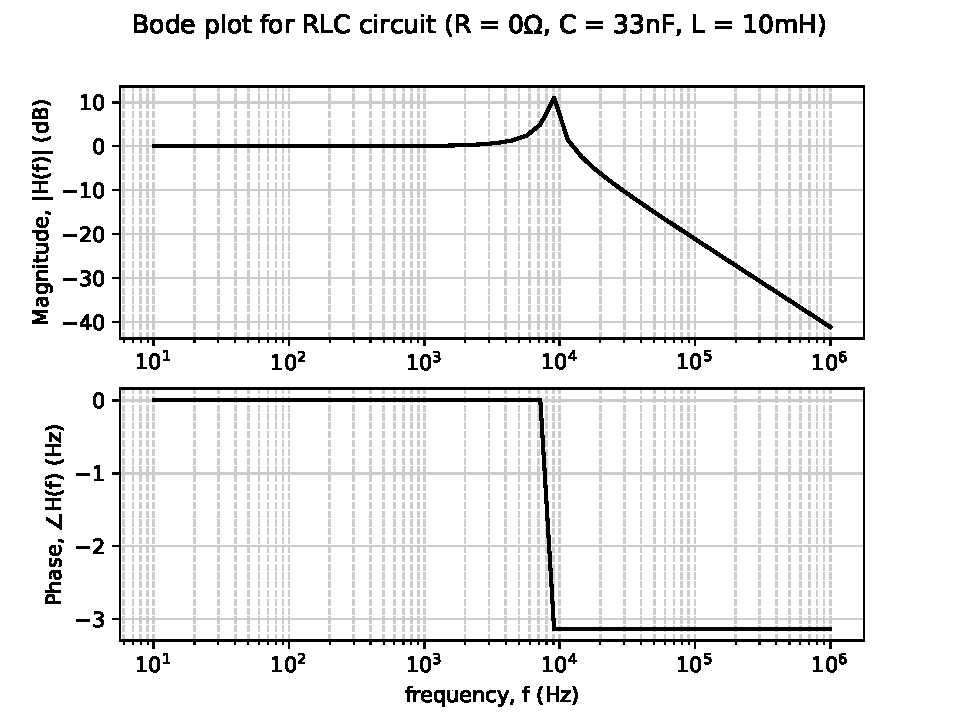
\includegraphics[width=0.76\textwidth]{plots/fig/Q2_c_RCL_0_freq.pdf}
  \caption{Plot of $|H(f)|$ with $R = 0\,\Omega$, $L=10\,mH$ and $C=33\,nF$ for $ 1\,Hz \le t \le 1\,MHz$.} 
  \label{fig:RLC_0_freq}
\end{figure}
%========================================RLC_0=End=======================================

%========================================RLC_22=Begin======================================
\subsubsection{RLC with $R_{RLC} = 22\,\Omega$, $C=33\,nF$ and $L=10\,mH$} 
Here $\alpha = 1100$ and $\omega_0 = 55\,048.2$. This is an underdamped response($\alpha < \omega_0$), which yields
\begin{equation}
  \label{eqn:rlc_22_ht_sub_intermediate}
  h(t) = \frac{1}{\sqrt{\tfrac{1}{(0.01)(33 \times 10^{-9})} - \left(\tfrac{22}{0.01}\right)^2}} \mathrm{e}^{-\tfrac{22}{0.01} t} \sin\!\Bigg(\sqrt{\tfrac{1}{(0.01)(33 \times 10^{-9})} - \left(\tfrac{22}{0.01}\right)^2} \, t\Bigg) u(t).
\end{equation}
The equation then simplifies to:
\begin{equation}
  \label{eqn:rlc_22_ht_sub}
  h(t) = 18.1804 \times 10^{_6} \mathrm{e}^{-2200 \, t} \sin\!\Bigg(55004.21 \, t\Bigg) u(t).
\end{equation}
This results in a decaying sinosoidal graph in Figure \ref{fig:RLC_22_time}. This behaviour is due to small non-zero resistance $R$ which dissipates some power, but not enough to immediately counteract the oscilation between the capacitor and inductor.
\begin{figure}[H]
  \centering
  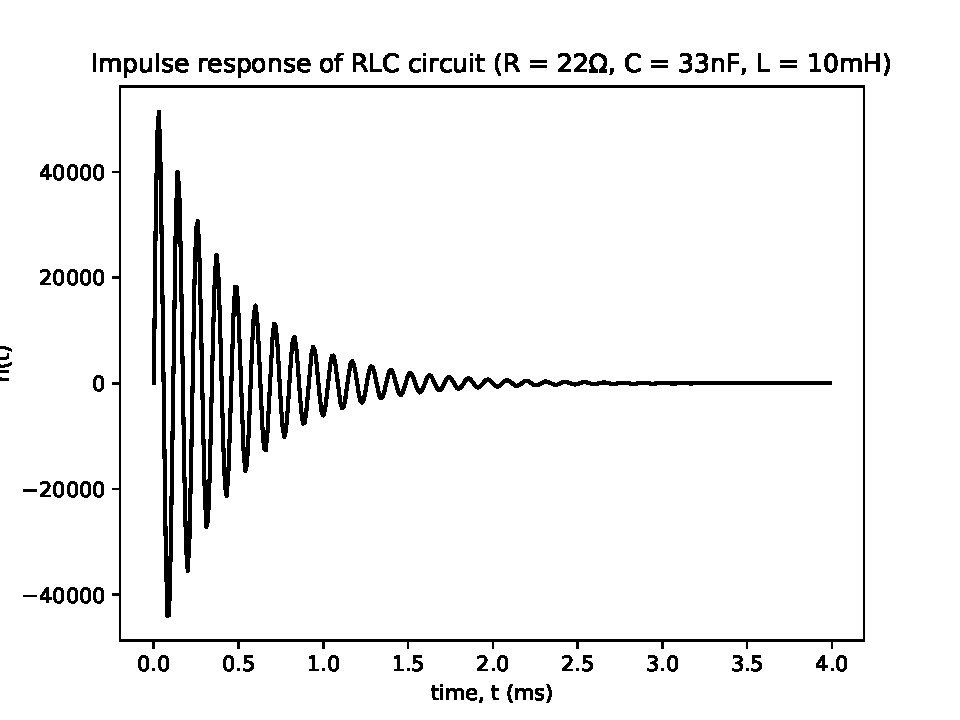
\includegraphics[width=0.76\textwidth]{plots/fig/Q2_d_RCL_22_time.pdf}
  \caption{Plot of $h(t)$ with $R = 22\,\Omega$, $L=10\,mH$ and $C=33\,nF$ for $ 0 \le t \le 4 \, ms$.}
  \label{fig:RLC_22_time}
\end{figure}
The frequency response in this case is
\begin{equation}
  \label{eqn:rlc_22_Hf_sub}
    |H(f)| = \frac{1}{\sqrt{ \left( 1 - (2 \pi f)^2 (0.01)(33 \times 10^{-9}) \right)^2 + (2 \pi f (22)(33 \times 10^{-9}))^2 }}.
\end{equation}
Plotting this equation results in a similar graph (Figure \ref{fig:RLC_22_freq}) previously seen, but a notable difference is the smoother transitions in the phase spectrum.
\begin{figure}[H]
  \centering
  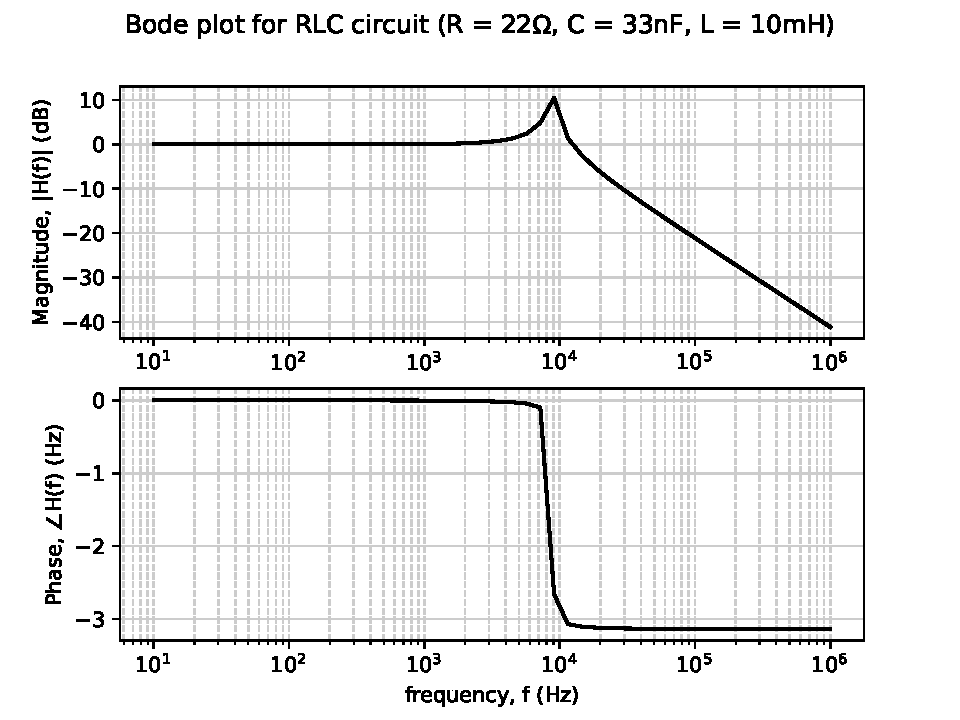
\includegraphics[width=0.76\textwidth]{plots/fig/Q2_d_RCL_22_freq.pdf}
  \caption{Plot of $|H(f)|$ with $R = 0\,\Omega$, $L=10\,mH$ and $C=33\,nF$ for $ 1\,Hz \le t \le 1\,MHz$.} 
  \label{fig:RLC_22_freq}
\end{figure}
%========================================RLC_22=End======================================

\subsubsection{RLC with $R_{RLC} = 680\,\Omega$, $C=33\,nF$ and $L=10\,mH$}  
Firstly, $\alpha$ and $\omega_0$ was calculated to be $34\,000\,$Np/s and $55\,048.2\,$rad/s, respectively. It is clear that $\alpha$ is much smaller than $\omega_0$, so this system is underdamped. This means that 
\begin{equation}
  h(t) = \frac{\omega_0}{\sqrt{1-\zeta^2}}\mathrm{e}^{-\alpha t}\operatorname{sin}(\omega_dt),
\end{equation}
where $\zeta$ is the damping coefficient given by $\frac{\alpha}{\omega_0}$, and $\omega_d$ is the damped natural frequency by $\omega_0\sqrt{1-\zeta^2}$. Their values were calculated to be $0.618$ and $43\,293.24$, respectively, leading to 
\begin{equation}
  h(t) = 70\,024.3\mathrm{e}^{-34\,000t}\operatorname{sin}(43\,293.24t),
\end{equation}
simplified. This expression for $h(t)$ is then plotted for 0 to $300\,\mu s$ in Figure \ref{fig:RLC_680_time}.
\begin{figure}[H]
  \centering
  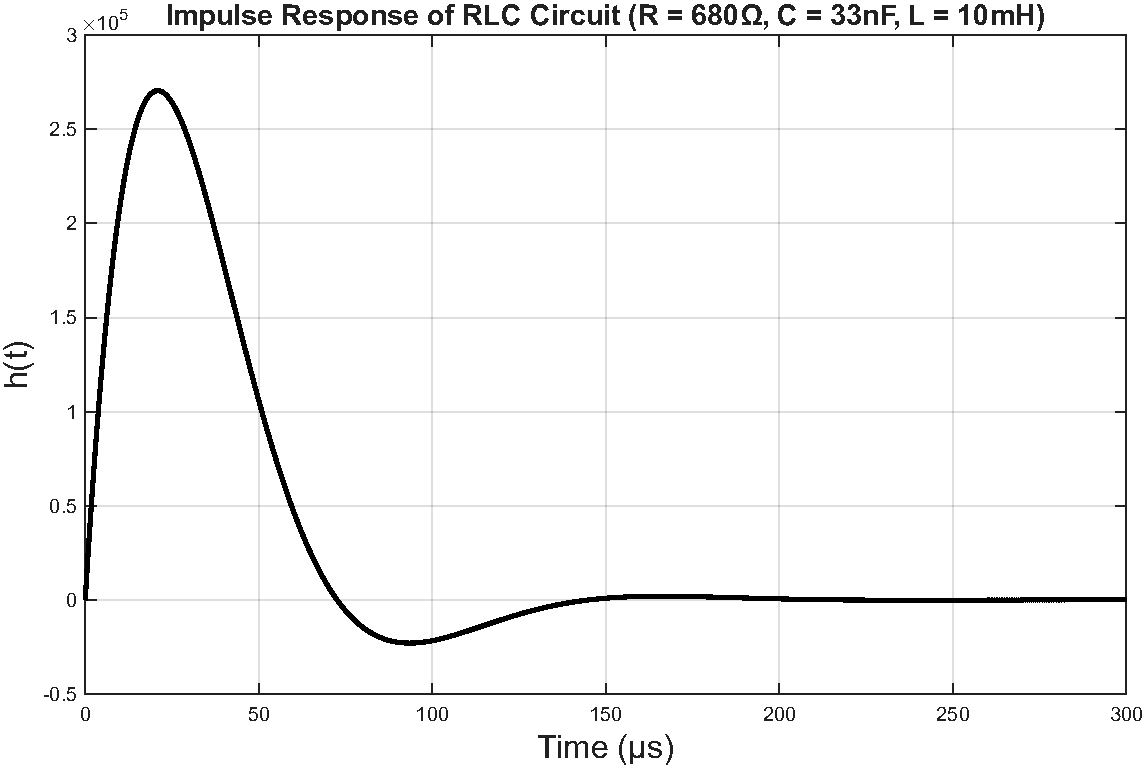
\includegraphics[width=0.76\textwidth]{plots/Q2e_ht_plot.pdf}
  \caption{Plot of $h(t)$ with $R = 680\,\Omega$, $L=10\,mH$ and $C=33\,nF$ for $ 0 \le t \le 4 \, ms$.}
  \label{fig:RLC_680_time}
\end{figure}
Furthermore, the transfer function can be found by simply substituting the given values into (\ref{eqn:rlc_Hf_general}):
\begin{equation}
  |H(f)| = \frac{1}{\sqrt{(1-3.95 \times 10^{-9}f^2)^2+19.88\times 10^{-9}f^2}}.
\end{equation}
This result is then plotted for $1\,Hz\leq f \leq 1\, MHz$ on a logarithmic scale in Figure \ref{fig:RLC_680_freq}.
\begin{figure}[H]
  \centering
  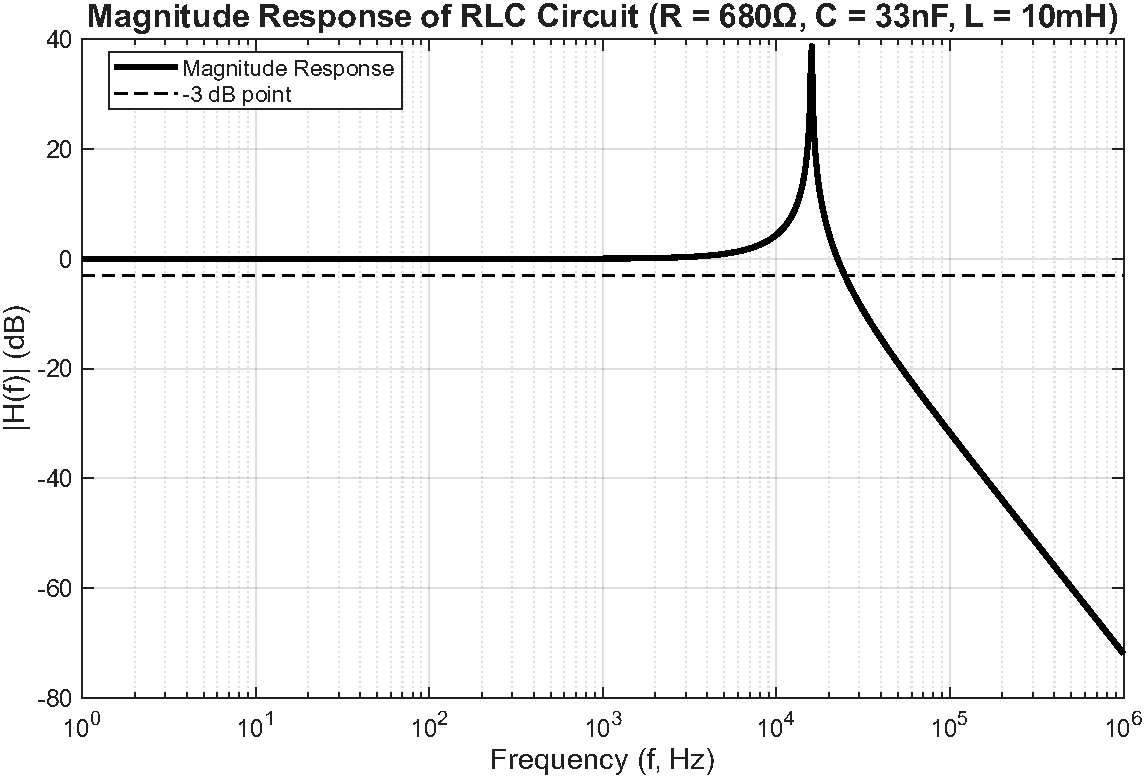
\includegraphics[width=0.76\textwidth]{plots/Q2e_Hf_plot.pdf}
  \caption{Plot of $|H(f)|$ with $R = 680\,\Omega$, $L=10\,mH$ and $C=33\,nF$ for $ 1\,Hz \le t \le 1\,MHz$.} 
  \label{fig:RLC_680_freq}
\end{figure}

The above figure shows the resonant frequency of approximately $40\,dB$. This sudden increase correlates to a larger $Q$-value. The circuit is also close to being critically damped, as the cusp is much sharper and close to being flattened.

\subsubsection{RLC with $R_{RLC} = 10\,k\Omega$, $C=33\,nF$ and $L=10\,mH$}
Following the same procedure as previously, $\alpha$ is determined to be $500\,000$ and $\omega_0$, $55\,048.2$. Now $\alpha$ is greater than $\omega_0$ and the system is overdamped, so it is necessary to find the characteristic roots ($s_1$ and $s_2$). By (\ref{char_roots}), they are found to be $-3\,039.54$ and $-996\,960.5$, respectively. Next the coefficients are required, and for this the LaPlace Transform is employed:
\begin{align}
  H(s) &= \mathscr{L} \{h(t)\} \nonumber\\ 
       &= \frac{1}{s^2LC+sRC +1} \\ 
  \implies sH(s) &= \mathscr{L} \{h'(t)\}
\end{align}
then 
\begin{align}
  h(0^+) &= \lim_{s \to \infty} sH(s) \nonumber\\ 
         &= 0
\end{align} 
and 
\begin{align}
  h'(0^+) &= \lim_{s \to \infty} s^2H(s) \nonumber\\ 
          &= \frac{1}{LC} \nonumber\\ 
          &= 3\,030\,303\,030.
\end{align}
Using these results to set up simultaneous equations, $A$ and $B$ are solved to be $3\,048.8$ and $-3\,048.8$, respectively. Finally
\begin{equation}
  h(t) = 3\,048.8 \mathrm{e}^{-3\,039.54t} -3\,048.8 \mathrm{e}^{-996\,960,5t},
\end{equation}
and plotted over a time period of $0 \leq t \leq 3\,ms$ in Figure \ref{fig:RLC_10k_time}
\begin{figure}[H]
  \centering
  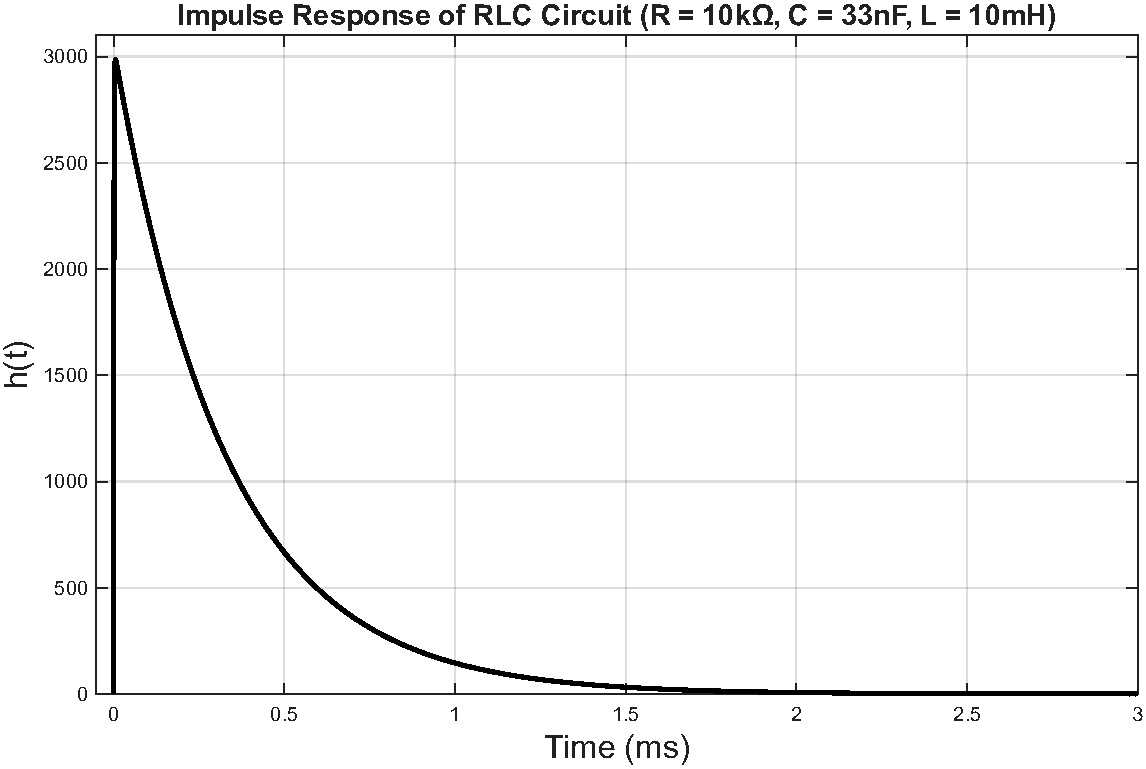
\includegraphics[width=0.76\textwidth]{plots/Q2f_ht_plot.pdf}
  \caption{Plot of $h(t)$ with $R = 10\,k\Omega$, $L=10\,mH$ and $C=33\,nF$ for $ 0 \le t \le 4 \, ms$.}
  \label{fig:RLC_10k_time}
\end{figure}
Finally substituting the given values into (\ref{eqn:rlc_Hf_general}) yields
\begin{equation}
  |H(f)| = \frac{1}{\sqrt{(1-13.03 \times 10^{-9}f^2)^2 + 4.3 \times 10^{-6}f^2}}.
\end{equation}
The above is then plotted on a logarithmic scale for $1\,Hz\leq f \leq 1\, MHz$ in Figure \ref{fig:RLC_10k_freq}.
\begin{figure}[H]
  \centering
  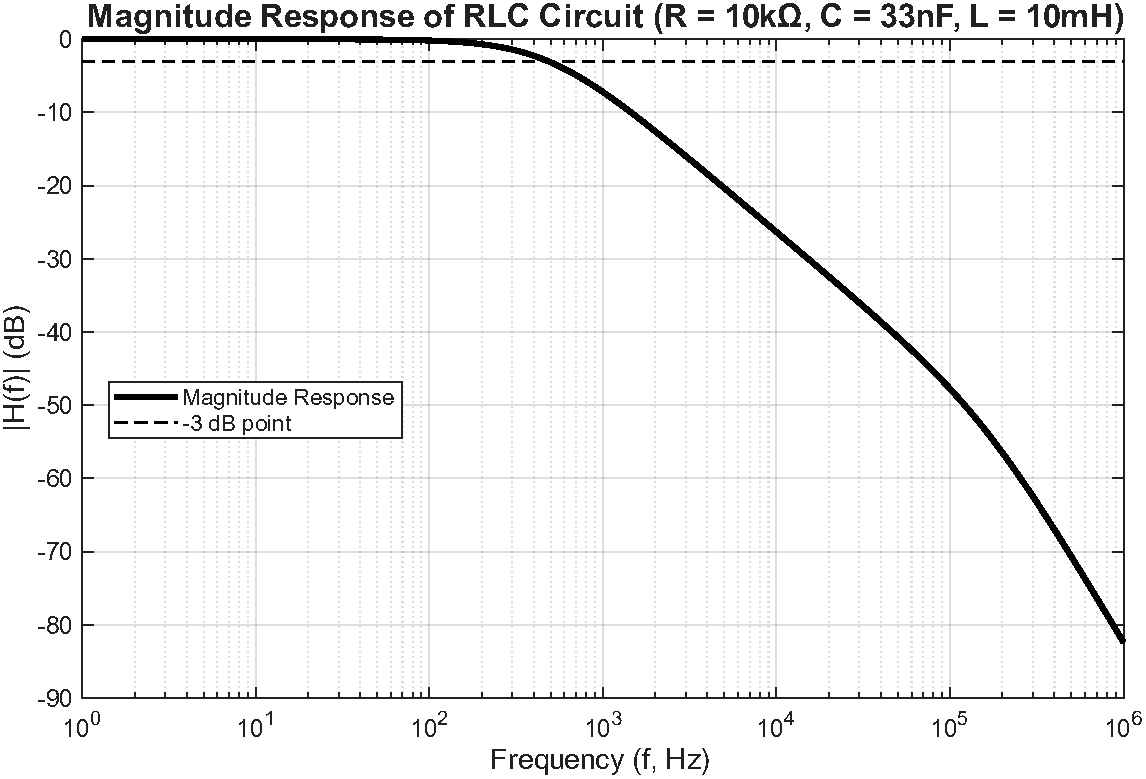
\includegraphics[width=0.76\textwidth]{plots/Q2f_Hf_plot.pdf}
  \caption{Plot of $|H(f)|$ with $R = 10\,k\Omega$, $L=10\,mH$ and $C=33\,nF$ for $ 1\,Hz \le t \le 1\,MHz$.} 
  \label{fig:RLC_10k_freq}
\end{figure}

Here the cusp is completely flattened, correlating to an overdamped circuit and a low $Q$-value. The RLC circuit essentially loses its selective band-pass behavior and begins behaving closer to a simple RC low-pass (since the resistor dominates). So, it can be concluded that as the resistance in each RLC circuit increases, the passband widens. 


\newpage
\section{Practical Results}
\label{sec:prac_results}

The signal generator circuit was constructed according to the diagram in Figure \ref{fig:Signal_Gen_Circuit}. 
To minimise parasitic effects, resistors were directly connected between nodes rather than using long wires, thereby reducing stray capacitance and inductance. 
The first measurements were taken with $R = 10 \, k\Omega$.

\begin{figure}[H]
  \centering
  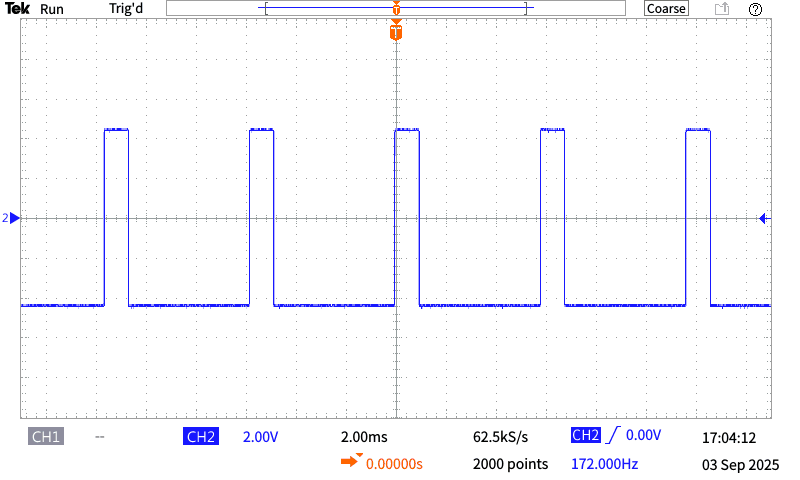
\includegraphics[width=0.8\textwidth]{scope/SigGen_10k_time.PNG}
  \caption{Signal generator circuit time-domain response with resistance value of $10\,k\Omega$}
  \label{fig:practical_signal_10k_time}
\end{figure}

The time-domain response of the signal generator (Figure \ref{fig:practical_signal_10k_time}) indicates a duty cycle of approximately $20\%$. 
FFT analysis was then performed using the oscilloscope, as shown in Figure \ref{fig:practical_signal_10k_fft}.


\begin{figure}[H]
  \centering
  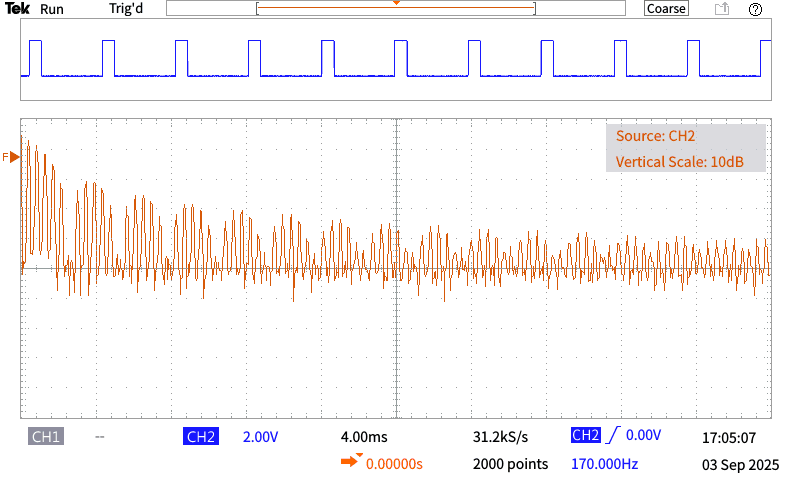
\includegraphics[width=0.8\textwidth]{scope/SigGen_10k_FFT.PNG}
  \caption{Signal generator circuit frequency-domain response with resistance value of $10\,k\Omega$}
  \label{fig:practical_signal_10k_fft}
\end{figure}

The FFT spectrum exhibits broad frequency content, which is advantageous for characterising filter behaviour. 
The resistor was then changed to $R = 1 \, k\Omega$, yielding the following responses:

\begin{figure}[H]
  \centering
  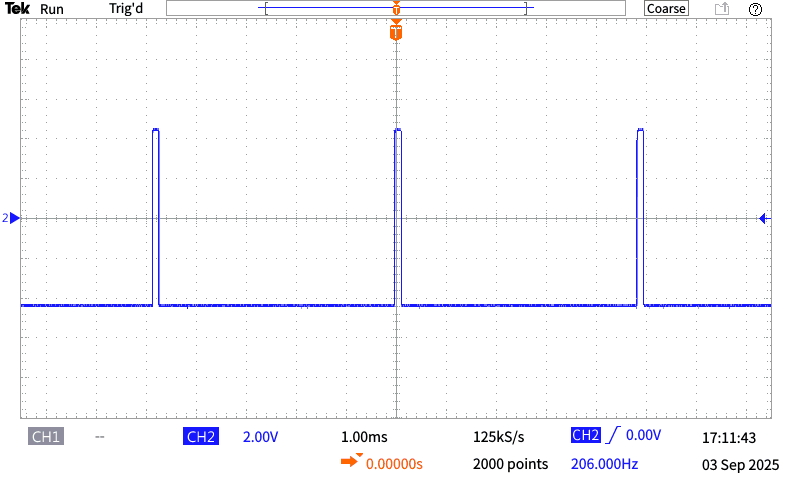
\includegraphics[width=0.8\textwidth]{scope/SigGen_1k_time.PNG}
  \caption{Signal generator circuit time-domain response with resistance value of $1k\Omega$} %Fix L  A  B  E  L
  \label{fig:practical_signal_1k_time}
\end{figure}

\begin{figure}[H]
  \centering
  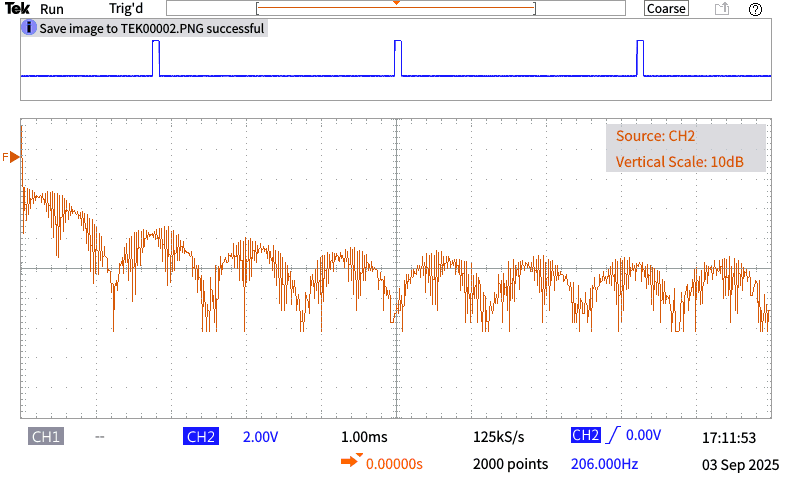
\includegraphics[width=0.8\textwidth]{scope/SigGen_1k_FFT.PNG}
  \caption{Signal generator circuit frequency-domain response with resistance value of $1k\Omega$} %Fix label
  \label{fig:practical_signal_1k_fft}
\end{figure}

With $R = 1 \, k\Omega$, the duty cycle decreases significantly to about $5\%$. 
The FFT response reveals additional frequency components, producing a denser spectral distribution that enhances the usefulness of the signal for filter testing.

A series RC circuit was then implemented as a low-pass filter, with the output measured across the capacitor. 
The results are shown below:

\begin{figure}[H]
  \centering
  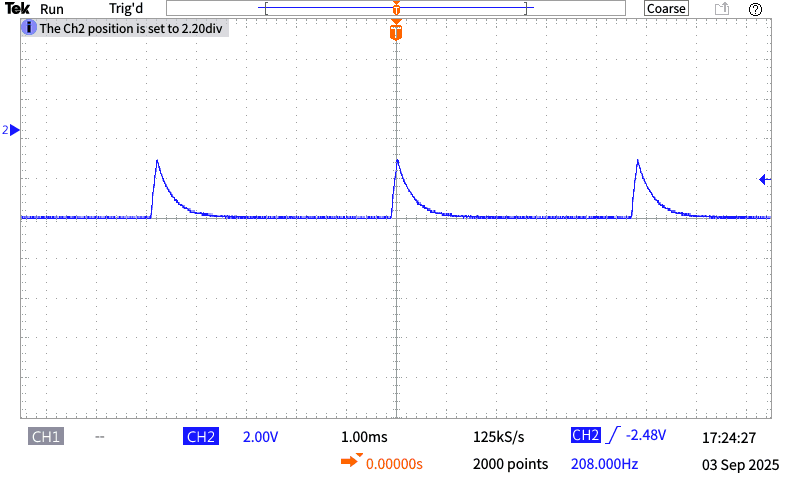
\includegraphics[width=0.8\textwidth]{scope/RC_time.PNG}
  \caption{Time-domain output of the RC circuit} %I know these labels are wrong I will fix them later
  \label{fig:RC_Time}
\end{figure}

\begin{figure}[H]
  \centering
  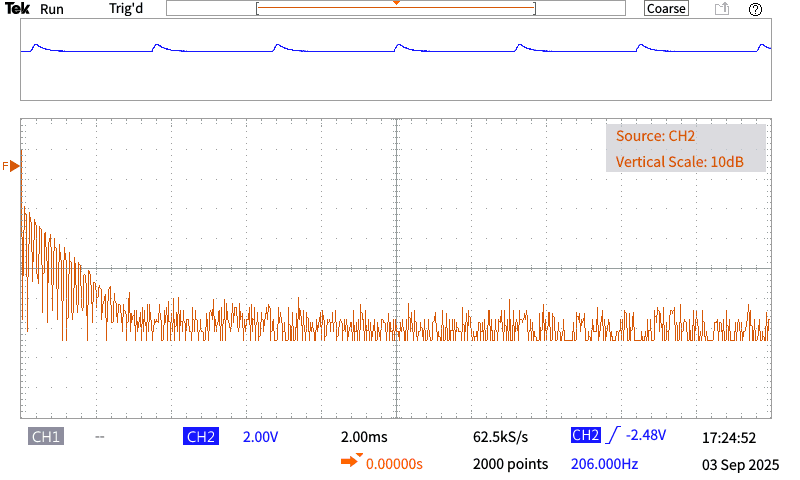
\includegraphics[width=0.8\textwidth]{scope/RC_FFT.PNG}
  \caption{FFT of the RC circuit} %here too
  \label{fig:RC_FFT}
\end{figure}

The capacitor discharge is evident in Figure \ref{fig:RC_Time}, while the FFT (Figure \ref{fig:RC_FFT}) clearly demonstrates attenuation of high-frequency components compared to the signal generator spectrum in Figure \ref{fig:practical_signal_1k_fft}. 
This behaviour confirms the expected low-pass filter action.

A series RL circuit was next configured as a high-pass filter, with the output measured across the resistor. 
The results are shown in Figures \ref{fig:RL_Time} and \ref{fig:RL_FFT}.

\begin{figure}[H]
  \centering
  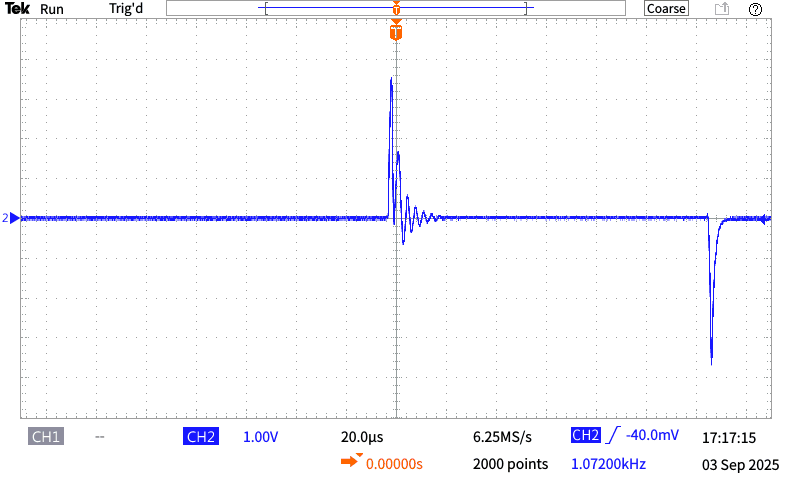
\includegraphics[width=0.8\textwidth]{scope/RL_time.PNG}
  \caption{FFT of the RL circuit} %here too
  \label{fig:RL_Time}
\end{figure}

\begin{figure}[H]
  \centering
  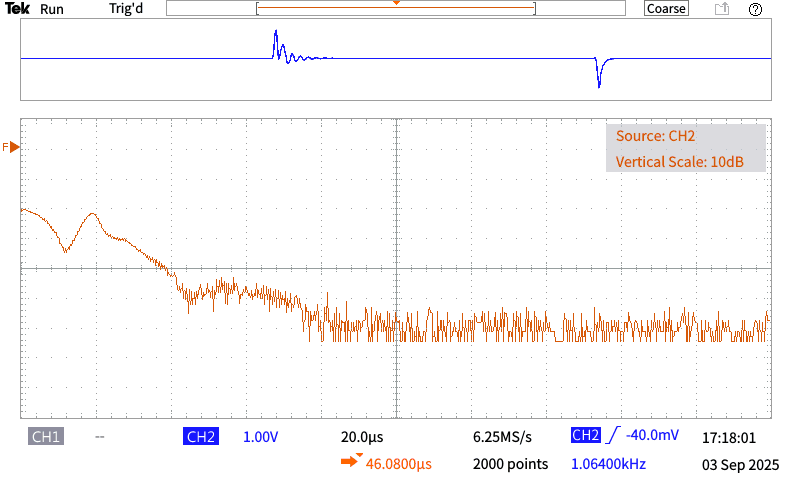
\includegraphics[width=0.8\textwidth]{scope/RL_FFT.PNG}
  \caption{FFT of the RL circuit} %here too
  \label{fig:RL_FFT}
\end{figure}

The measured time-domain response (Figure \ref{fig:RL_Time}) exhibited unexpected behaviour, which persisted across multiple measurement attempts with different components. 
This anomaly will be analysed further in Section \ref{sec:discussion}. 
Nonetheless, the FFT results confirm that the RL circuit primarily passes higher frequencies, consistent with theoretical predictions.

Finally, a series RLC circuit was tested as a band-pass filter, beginning with $R = 0 \, \Omega$. 
The resulting plots are presented in Figures \ref{fig:RLC_Time} and \ref{fig:RLC_FFT}.

\begin{figure}[H]
  \centering
  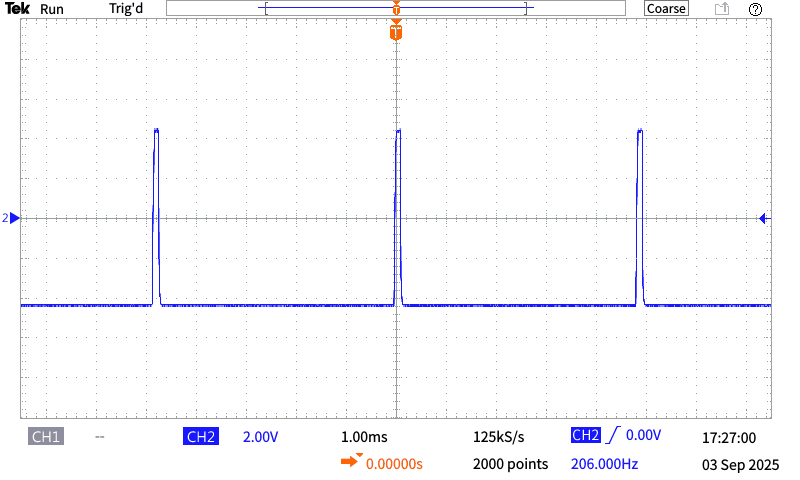
\includegraphics[width=0.8\textwidth]{scope/RLC_0_time.PNG}
  \caption{RLC circuit time-domain response with resistance value of $0\,\Omega$} %here too
  \label{fig:RLC_Time}
\end{figure}

\begin{figure}[H]
  \centering
  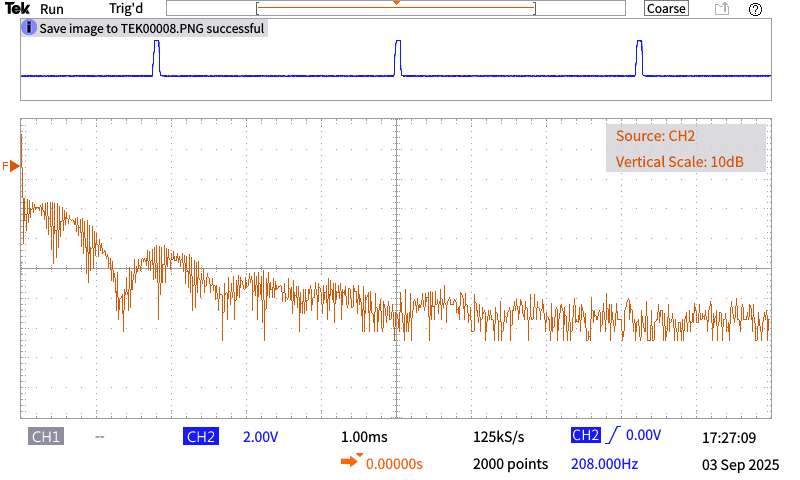
\includegraphics[width=0.8\textwidth]{scope/RLC_0_FFT.PNG}
  \caption{RLC circuit FFT with resistance value of $0\,\Omega$} %here too
  \label{fig:RLC_FFT}
\end{figure}

The observed results deviate significantly from theoretical expectations. 
A band-pass filter should attenuate both very low and very high frequencies while allowing a narrow band to pass \cite{lathi}, but this behaviour was not clearly observed. 
The circuit was subsequently tested with higher resistance values ($22 \, \Omega$, $680 \, \Omega$, and $10 \, \text{k}\Omega$), with the results shown in Figures \ref{fig:RLC22_Time} to \ref{fig:RLC10k_FFT}.  

\begin{figure}[H]
  \centering
  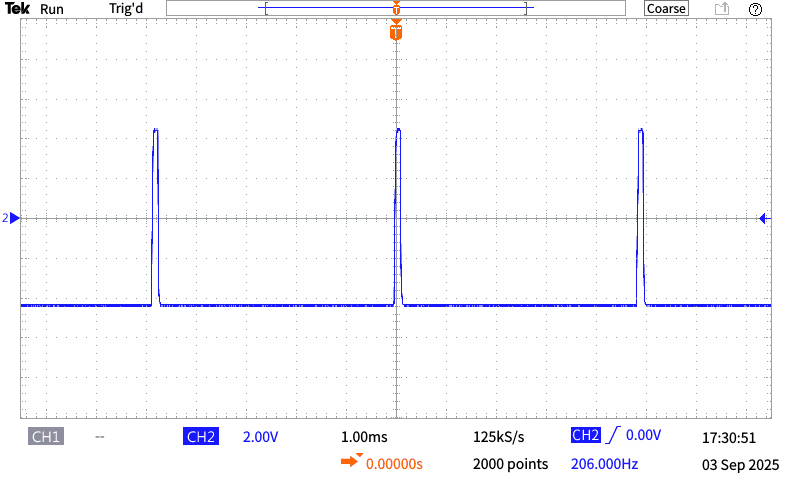
\includegraphics[width=0.8\textwidth]{scope/RLC_22_time.PNG}
  \caption{RLC circuit time-domain response with resistance value of $22\,\Omega$} %here too
  \label{fig:RLC22_Time}
\end{figure}

\begin{figure}[H]
  \centering
  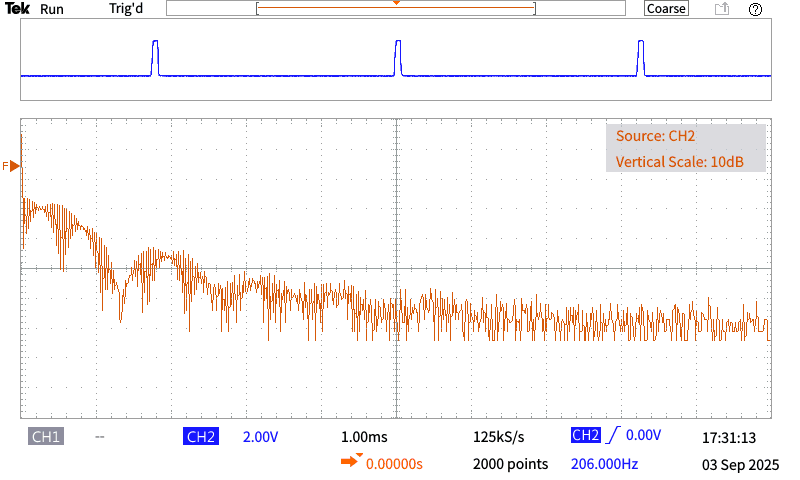
\includegraphics[width=0.8\textwidth]{scope/RLC_22_FFT.PNG}
  \caption{RLC circuit with resistance value of $22\,\Omega$ FFT} %here too
  \label{fig:RLC22_FFT}
\end{figure}


\begin{figure}[H]
  \centering
  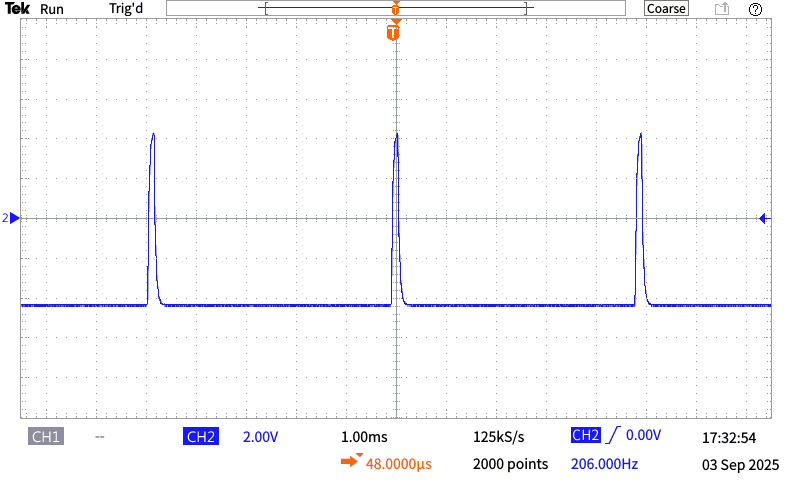
\includegraphics[width=0.8\textwidth]{scope/RLC_680_time2.PNG}
  \caption{RLC circuit time-domain response with resistance value of $680\,\Omega$} %here too
  \label{fig:RLC680_Time}
\end{figure}

\begin{figure}[H]
  \centering
  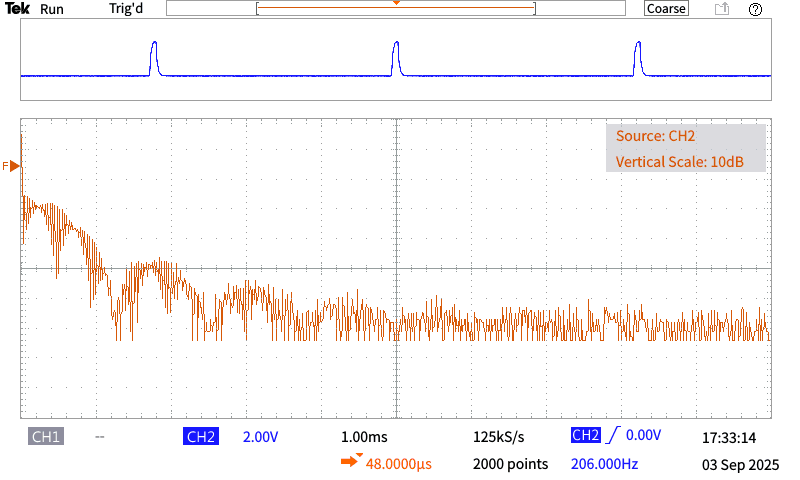
\includegraphics[width=0.8\textwidth]{scope/RLC_680_FFT.PNG}
  \caption{RLC circuit with resistance value of $680\,\Omega$ FFT} %here too
  \label{fig:RLC680_FFT}
\end{figure}


\begin{figure}[H]
  \centering
  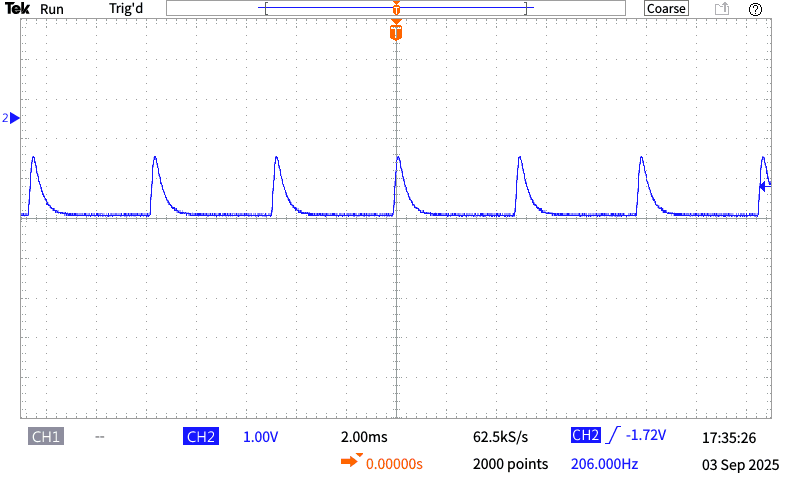
\includegraphics[width=0.8\textwidth]{scope/RLC_10k_time.PNG}
  \caption{RLC circuit time-domain response with resistance value of $10\,k\Omega$} %here too
  \label{fig:RLC10k_Time}
\end{figure}

\begin{figure}[H]
  \centering
  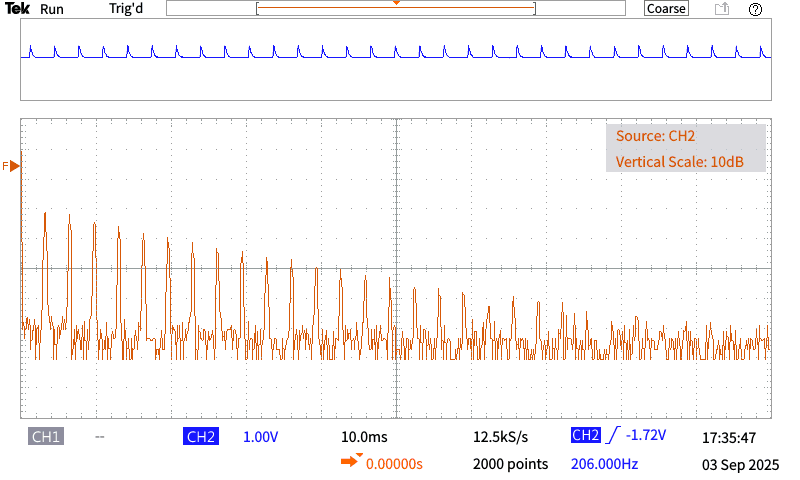
\includegraphics[width=0.8\textwidth]{scope/RLC_10k_FFT.PNG}
  \caption{RLC circuit with resistance value of $10\,k\Omega$ FFT} %here too
  \label{fig:RLC10k_FFT}
\end{figure}

At low and medium resistance values, the experimental responses continued to diverge from the theoretical predictions. 
However, at $R = 10 \, \text{k}\Omega$, the measured time-domain output (Figure \ref{fig:RLC10k_Time}) shows an overdamped response consistent with theory, and the corresponding FFT (Figure \ref{fig:RLC10k_FFT}) better matches the expected wide passband. 
This suggests that circuit parasitics and component tolerances had a significant impact on the behaviour of the lower-resistance RLC configurations.

\newpage
\section{Discussion}
\label{sec:discussion}

To validate the experimental results, LTSpice simulations were conducted using the \textit{TL064CN} op-amp model obtained from Texas Instruments \cite{ti2025homepage}. 
The simulation setup for the signal generator circuit is shown in Figure \ref{fig:Signal_Gen_Circuit}.

\begin{figure}[H]
  \centering
  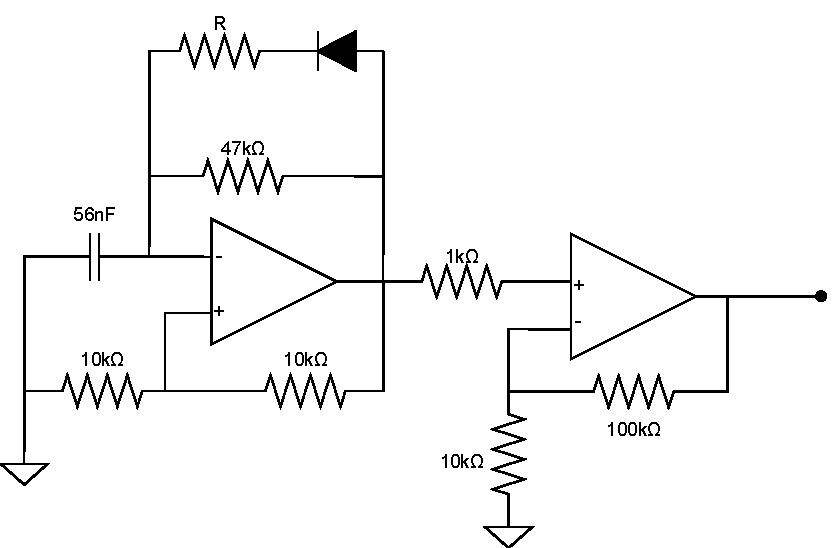
\includegraphics[width=0.8\textwidth]{Figures/SignalGenCircuit.pdf}
  \caption{Signal generator circuit setup in LTSpice}
  \label{fig:Signal_Gen_Circuit}
\end{figure}

Simulations were first run without a load to establish the baseline impulse train. 

Due to discrepancies observed in the practical measurements, comparisons focus primarily on the period of the signals, since this quantity remains well defined even when the waveform shape is distorted.

The period $T_0 = 2\pi \sqrt{LC}$ directly determines the resonant frequency and is therefore a critical metric for evaluating filter behaviour \cite{lathi}. 
By comparing simulated and measured periods, the influence of parasitics and component tolerances can be quantified.  

For $R = 10 \, k\Omega$, the simulated period was $3.4 \, \text{ms}$ compared to a measured $5.8 \, \text{ms}$ (a $70\%$ increase). 
The discrepancy is attributed to parasitic capacitance from the breadboard and wiring, as well as component tolerances ($\pm 5\%$ for resistors, $\pm 10$–$20\%$ for capacitors). 

A similar trend was observed with $R = 1 \, \text{k}\Omega$, where the simulated period was $2.9 \, \text{ms}$ and the measured period $4.8 \, \text{ms}$, again representing a $65\%$ increase.  


\begin{figure}[H]
  \centering
  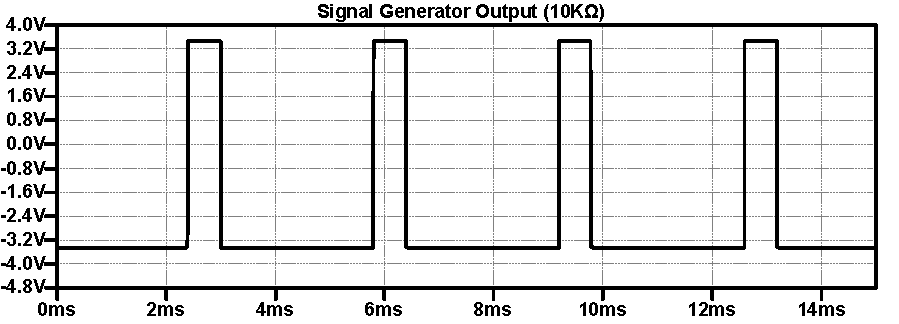
\includegraphics[width=0.8\textwidth]{Figures/10k_func_gen.pdf}
  \caption{Simulated time-domain output of the signal generator with $10\,k\Omega$} 
  \label{fig:Signal_Gen_10k}
\end{figure}

\begin{figure}[H]
  \centering
  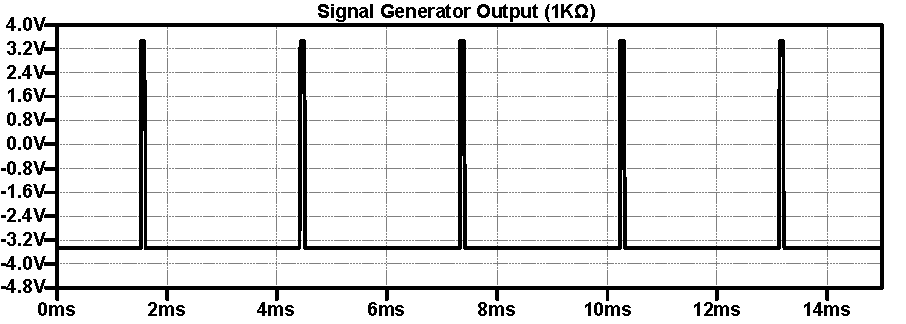
\includegraphics[width=0.8\textwidth]{Figures/1k_func_gen.pdf}
  \caption{Simulated time-domain output of the signal generator with $1\,k\Omega$}
  \label{fig:Signal_Gen_1k}
\end{figure}

For the RC circuit, the simulated and measured time responses had nearly identical shapes, but the same $65$–$70\%$ period discrepancy persisted (Figures \ref{fig:Sim_RC} and \ref{fig:RC_Time}). 

This indicates that while the low-pass filtering behaviour is correct, the cutoff frequency is shifted downward in practice, consistent with increased capacitance in the physical setup.

\begin{figure}[H]
  \centering
  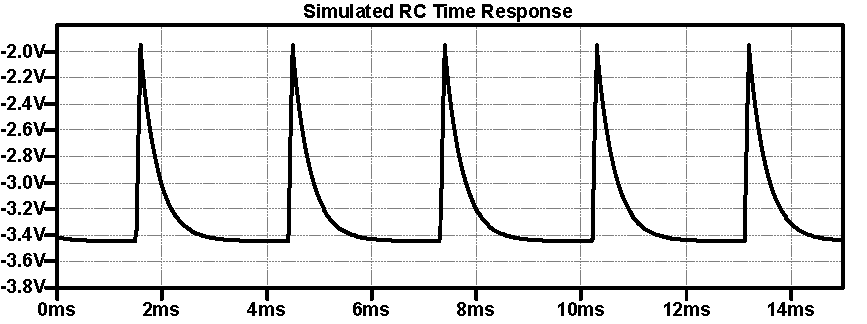
\includegraphics[width=0.8\textwidth]{Figures/RC_SIM.pdf}
  \caption{Simulated time-domain output of the RC circuit}
  \label{fig:Sim_RC}
\end{figure}

For the RL circuit, simulations showed the expected clean high-pass response (Figure \ref{fig:Sim_RL}). 
In contrast, the measured response (Figure \ref{fig:RL_Time}) displayed oscillatory behaviour resembling an underdamped system, again pointing to significant parasitic capacitance on the breadboard. 
The period difference between simulation and experiment was smaller here (around $60\%$), likely due to the dominance of the $10 \, \text{mH}$ inductor in setting the time constant.

\begin{figure}[H]
  \centering
  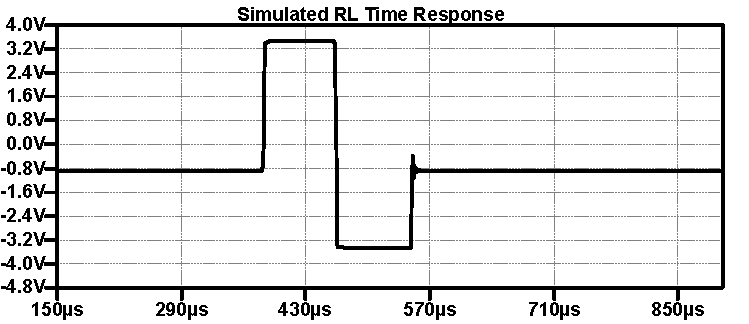
\includegraphics[width=0.8\textwidth]{Figures/RL_Sim.pdf}
  \caption{Simulated time-domain output of the RL circuit}
  \label{fig:Sim_RL}
\end{figure}

For the RLC circuits, simulations confirmed that varying the value of $R$ alters the damping while leaving the oscillation period unchanged (since $L$ and $C$ are fixed). 
At $R = 0 \, \Omega$, the circuit was highly underdamped (Figure \ref{fig:Sim_RLC_0}). 
With $R = 22 \, \Omega$, the oscillations decayed more rapidly, while $R = 680 \, \Omega$ produced a response approaching critical damping (Figures \ref{fig:Sim_RLC_22} and \ref{fig:Sim_RLC_680}). 
Finally, with $R = 10 \, k\Omega$, the response became overdamped (Figure \ref{fig:Sim_RLC_10k}).  

These observations match theoretical expectations:
\begin{enumerate}
    \item \textbf{Low resistance case} ($R = 0\,\Omega$):
    \begin{itemize}
        \item Exhibits a narrow, selective passband characteristic
        \item Demonstrates underdamped behavior
    \end{itemize}
    
    \item \textbf{High resistance case} ($R = 10\,k\Omega$):
    \begin{itemize}
        \item Displays a broader passband characteristic
        \item Demonstrates overdamped behavior
    \end{itemize}
\end{enumerate}

The FFT analysis further illustrates this trend, showing that the $R = 0\,\Omega$ case produces a sharply peaked frequency response (narrow bandwidth), whereas the $R = 10\,k\Omega$ case exhibits a much broader passband, consistent with theoretical expectations \cite{lathi}.

\begin{figure}[H]
  \centering
  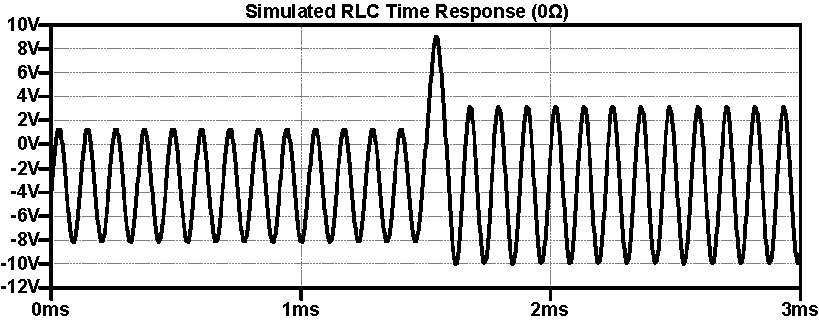
\includegraphics[width=0.8\textwidth]{Figures/0_RLC.pdf}
  \caption{Simulated time-domain output of the RLC circuit with $0\,\Omega$}
  \label{fig:Sim_RLC_0}
\end{figure}

\begin{figure}[H]
  \centering
  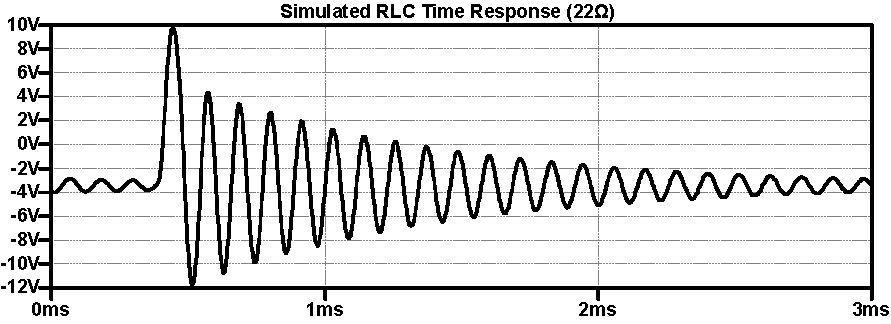
\includegraphics[width=0.8\textwidth]{Figures/22_RLC.pdf}
  \caption{Simulated time-domain output of the RLC circuit with $22\,\Omega$}
  \label{fig:Sim_RLC_22}
\end{figure}

\begin{figure}[H]
  \centering
  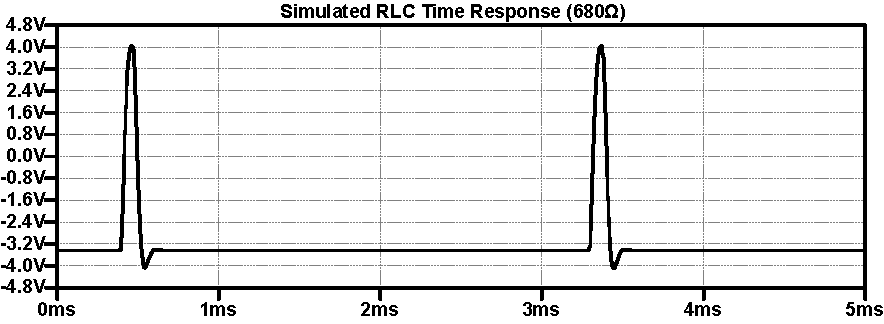
\includegraphics[width=0.8\textwidth]{Figures/680_RLC.pdf}
  \caption{Simulated time-domain output of the RLC circuit with $680\,\Omega$}
  \label{fig:Sim_RLC_680}
\end{figure}

\begin{figure}[H]
  \centering
  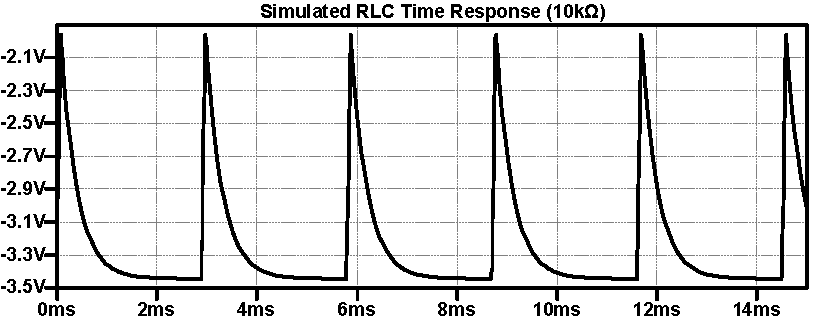
\includegraphics[width=0.8\textwidth]{Figures/10k_RLC.pdf}
  \caption{Simulated time-domain output of the RLC circuit with $10\,k\Omega$}
  \label{fig:Sim_RLC_10k}
\end{figure}

Overall, the discrepancies between simulated and measured results are explained primarily by non-idealities in the experimental setup, particularly parasitic capacitance and component tolerances. It was also realised that an inductor of a different value than $10\,mH$ was provided, also altering the measured results significantly.

Despite these differences, the qualitative behaviour of the RC, RL, and RLC circuits matched theoretical expectations, demonstrating their roles as low-pass, high-pass, and band-pass filters respectively.

Lastly a deeper discussion of the strange results observed in Section: \ref{sec:prac_results}. The following is the frequency response of the signal generator circuit with a resistance value of $1 \,k\Omega$:

\begin{figure}[H]
  \centering
  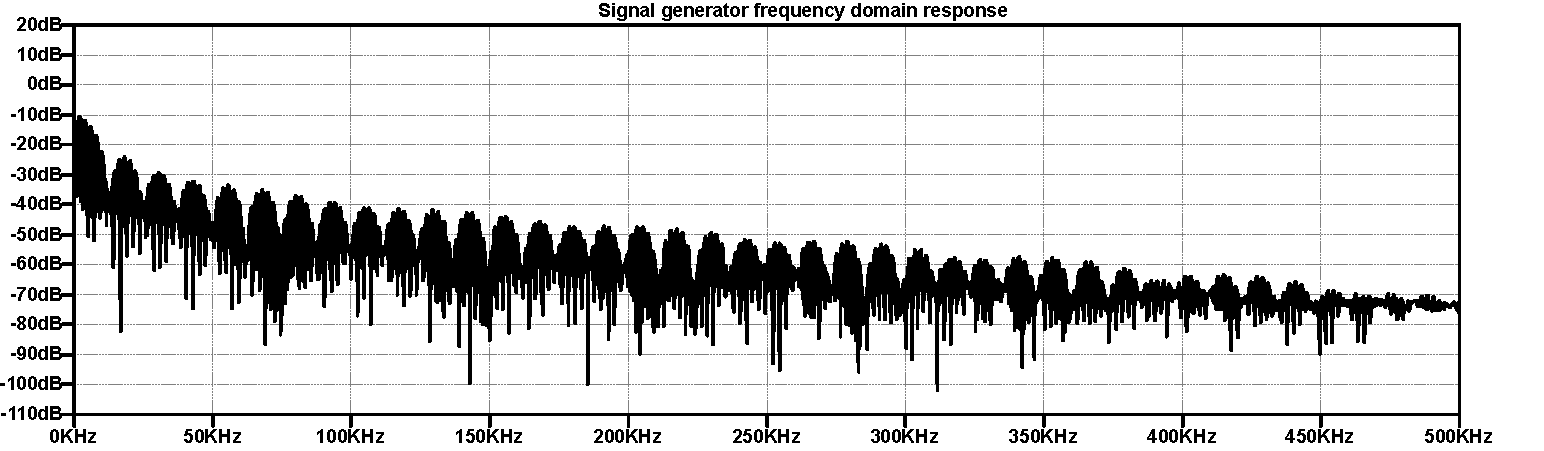
\includegraphics[width=0.8\textwidth]{Figures/SigGen1KFFT.pdf}
  \caption{Simulated frequency response of the signal generator with $1\, k\Omega$}
  \label{fig:FFT_SigGen_Sim}
\end{figure}

As discussed in Section \ref{sec:prac_results} the same wide range of frequencies are present making this an ideal set of test frequencies to study the response of these filters. The RLC, band-pass filter will spesifically be discussed to why it was stated in Section \ref{sec:prac_results} that the results are unexpected.

\begin{figure}[H]
  \centering
  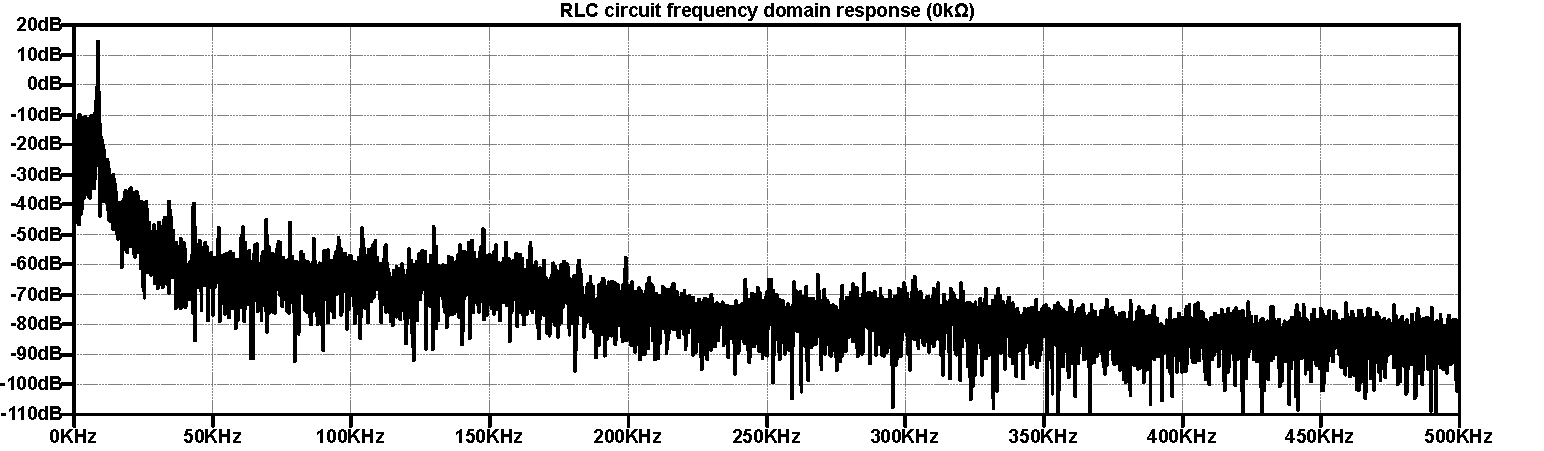
\includegraphics[width=0.8\textwidth]{Figures/RLC_0k_FFT_SIM.pdf}
  \caption{Simulated frequency response of the RLC circuit with $0 \,\Omega$}
  \label{fig:FFT_RLC0_Sim}
\end{figure}

The series RLC circuit with zero resistance exhibits extremely sharp frequency selectivity around its resonant frequency. Rather than providing smooth filtering, the lack of resistance allows the circuit to ring continuously when stimulated, causing the input frequency components to spread out due to sustained oscillatory behavior, i.e. the circuit is filtering, it is just doing so in a way that creates ringing and spectral spreading rather than clean frequency separation. 

Adding a $10 \, k\Omega$ resistor in series as discussed earlier yeilds the following frequency response:

\begin{figure}[H]
  \centering
  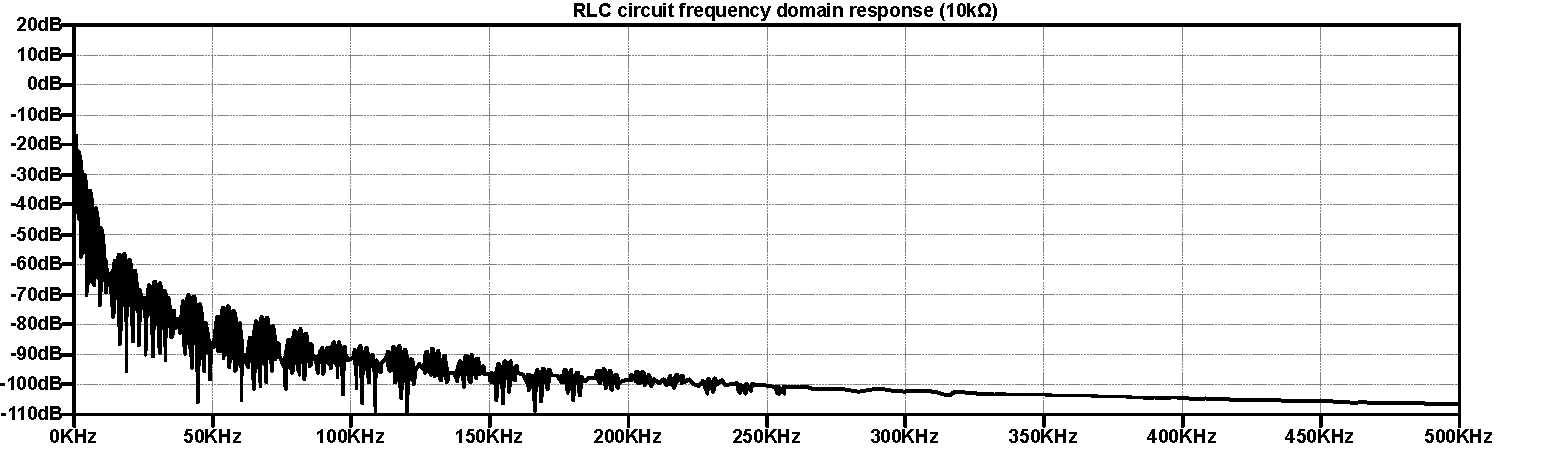
\includegraphics[width=0.8\textwidth]{Figures/RLC_10k_FFT_SIM.pdf}
  \caption{Simulated frequency response for the RLC circuit with $10 \,k\Omega$}
  \label{fig:FFT_RLC10k_Sim}
\end{figure}

Here it is evident that the pass-band created by the RLC circuit is relatively wide allowing a wide range of frequencies to pass. There is also a gradual roll off of the frequency band indicating that it isn't a very selective circuit. Lastly this circuit is greatly more stable than that of Figure \ref{fig:FFT_RLC0_Sim} with the high resistance value insuring that there is no ringing nor any oscillatory behaviour. Lastly due to the high resistance of the circuit the maximum amplituude of the response has been lowered. This circuit shows the opposite extreme of the previous one with maximum damping and broad frequency pass band.

The resistance in an RLC band-pass filter primarily controls the filter's bandwidth and selectivity. Higher resistance results in wider bandwidth (less selective filtering), while lower resistance produces narrower bandwidth (more selective filtering). This relationship is crucial when designing filters for different applications requiring specific bandwidth characteristics

\newpage

\section{Conclusion}
\label{sec:conclusion}
%WORK IN PROGRESS
This practical introduced the analysis of RC, RL, and RLC circuits in both the time and frequency domains. Through theoretical derivations, simulations, and experimental measurements, the frequency responses and impulse responses of these filters were obtained and compared. The results confirmed the expected filtering characteristics: attenuation of certain frequency ranges, phase behavior, and the effect of resistance on damping in RLC circuits. However, parasitic capacitance, tolerance effects and incorrectly provided components significantly influenced measured results, highlighting the importance of accounting for real-world non-idealities.

The Fourier analysis of a periodic pulse train demonstrated how pulse width influences the spectral content, while experimental oscilloscope measurements validated the theoretical predictions with minor deviations due to real-world component tolerances and measurement limitations. Overall, the practical achieved its objectives by reinforcing the connection between mathematical models, computational tools, and physical circuit behavior.


\newpage


% Make the reference font the same size as the rest of the text.
\IEEEtriggercmd{\normalsize}
\IEEEtriggeratref{1}

\bibliographystyle{IEEEtran}%
\bibliography{references}%



%\clearpage
\FloatBarrier


% Use for only one appendix (no titles necessary and no appendix numbers).
%\appendix
% Use for multiple appendices (with appendix numbers).
\newpage
\appendices


% \section{Abbreviations}
% \label{sec:abbreviations}

% \printglossary[type=\acronymtype]
\section{Code}
\label{app:code}

\subsubsection{Python script to generate figures for questions 1a,b and 2b,d}
\label{sec:code_q1_a_b_q2_b_d}
    \begin{mdframed}
        \inputminted{python}{./code/practical_2.py}
    \end{mdframed}

\subsubsection{MatLab code to generate figure of $C(f)$ with $\tau \to 0$}
\label{sec:code_q1_c}
    \begin{mdframed}
        \inputminted{Matlab}{./code/Q1c_Plot.m}
    \end{mdframed}

\subsubsection{MatLab code to generate figure of $h(t)$ with $R_{RLC} = 680\,\Omega$}
\label{sec:code_q2_e_ht}
    \begin{mdframed}
        \inputminted{Matlab}{./code/Q2e_ht_Plot.m}
    \end{mdframed}

\subsubsection{MatLab code to generate figure of $H(f)$ with $R_{RLC} = 680\,\Omega$}
\label{sec:code_q2_e_Hf}
    \begin{mdframed}
        \inputminted{Matlab}{./code/Q2e_Hf_Plot.m}
    \end{mdframed}

\subsubsection{MatLab code to generate plot for $h(t)$ with $R_{RLC} = 10\,k\Omega$}
\label{sec:code_q2_f_ht}
    \begin{mdframed}
        \inputminted{Matlab}{./code/Q2f_ht_Plot.m}
    \end{mdframed}

\subsubsection{MatLab code to generate plot for $H(f)$ with $R_{RLC} = 10\,k\Omega$}
\label{sec:code_q2_f_Hf}
    \begin{mdframed}
        \inputminted{Matlab}{./code/Q2f_Hf_Plot.m}
    \end{mdframed}


\end{document}
